\documentclass[12pt,a4paper]{report}
\usepackage[utf8]{inputenc}
\usepackage[T1]{fontenc}
\usepackage[arabic, french]{babel}
\usepackage{graphicx}
\usepackage{geometry}
\usepackage{setspace}
\usepackage{hyperref}
\usepackage{titlesec}
\usepackage{xcolor}
\geometry{margin=2.54cm}
\usepackage{array}
\usepackage{float}
\usepackage{makecell}
\usepackage{enumitem}
\usepackage{pgfplots} % Pour les graphiques
\pgfplotsset{compat=1.18} % Version stable

\usepackage{fancyhdr}
\usepackage{etoolbox} % Pour les corrections profondes

\makeatletter
% 1. Réinitialisation complète
\fancyhf{} % Efface tout
\renewcommand{\headrulewidth}{0pt} % Supprime la barre d'en-tête

% 2. Forçage du pied de page droit
\fancyfoot[R]{\vspace{-1cm}\thepage} % Ajustez le vspace au besoin

% 3. Correction pour les chapitres (classes book/report)
\patchcmd{\chapter}{\thispagestyle{plain}}{\thispagestyle{fancy}}{}{}
\makeatother

% ===== APPLICATION =====
\pagestyle{fancy} % Active le style


\doublespacing

\titleformat{\chapter}[display]
{\normalfont\bfseries\huge}{\chaptername\ \thechapter}{20pt}{\Huge}
\titleformat{\section}
{\normalfont\Large\bfseries}{\thesection}{1em}{}

\begin{document}
	 
	
	\pagenumbering{roman}   % numérotation romaine : i, ii, iii...
	
	\addcontentsline{toc}{chapter}{Dédicace}
	\chapter*{Dédicace}
	
	
	\begin{center}
		\begin{minipage}{0.8\textwidth} % Largeur contrôlée du texte
			\centering
			\Large\itshape % Style italique légèrement agrandi
			
			Je dédie ce travail à :\\[1.5em] % Espacement après la ligne
			
			Mes chers parents, mon frère,  \\
			pour leur sacrifice et leur motivation.\\[1em]
			
			À mon épouse et à ma petite fille,  \\
			qui m’apportent chaque jour la force pour avancer.\\[1em]
			
			À Mes amis \\
			pour leur contribution, qui a apporté une valeur ajoutée.\\[1em]
			
			À toute personne \\
			ayant contribué à ma formation.
			
		\end{minipage}
	\end{center}
	
	\clearpage
	\chapter*{Remerciement}
	\addcontentsline{toc}{chapter}{Remerciement}
			
	Au début, il m'est agréable d'exprimer ma reconnaissance à toute personne dont l'intervention au cours de ce stage a favorisé son aboutissement.\\
			
	Je tiens à remercier vivement mes encadrants, Monsieur \textsc{BERAHIOU Radwane} et Monsieur \textsc{Mouhib Imad}, pour leur temps précieux et le partage de leur expertise quotidienne. Leur confiance m'a permis de développer mes compétences de manière significative.\\[0.6em]
				
	Un grand merci à toute l'équipe d'\textsc{ALGOLUS} pour m'avoir offert cette opportunité de stage dans un environnement professionnel stimulant.\\[0.6em]
	
	Je tiens à exprimer ma sincère gratitude aux membres du jury pour le temps qu’ils ont consacré à l’évaluation de mon travail.\\[0.6em]
	
	Un remerciement particulier à \textsc{DOUHI Taoufik}, \textsc{ARRHIOUI Karim}, \textsc{ARRHIOUI Anass} et \textsc{BEREHIL Mohammed} pour leurs précieux conseils.\\[0.6em]
			
	Je remercie le corps professoral et administratif de l'\textsc{École des Hautes Études d'Ingénierie - Oujda} pour la qualité de la formation reçue.
	
	\clearpage
	\chapter*{Liste des abréviations}
	\addcontentsline{toc}{chapter}{Liste des abréviations}
	
	\begin{table}[H]
		\centering
		\begin{tabular}{|l|l|}
			\hline
			\textbf{Abréviation} & \textbf{Désignation} \\
			\hline
			API & Application Programming Interface \\
			\hline
			CPU & Central Processing Unit \\
			\hline
			HTTP & Hypertext Transfer Protocol \\
			\hline
			IDE & Integrated Development Environment \\
			\hline
			JDBC & Java Database Connectivity \\
			\hline
			JPA & Java Persistence API \\
			\hline
			LLM & Large Language Model \\
			\hline
			PDF & Portable Document Format \\
			\hline
			RAG & Retrieval-Augmented Generation \\
			\hline
			RAM & Random-Access Memory \\
			\hline
			SARL & Société À Responsabilité Limitée \\
			\hline
			SQL & Structured Query Language \\
			\hline
			SRP & Single Responsibility Principle \\
			\hline
			UML & Unified Modeling Language \\
			\hline
			URL & Uniform Resource Locator \\
			\hline
		\end{tabular}
		\label{tab:liste-abréviations}
	\end{table}
	
	
	\clearpage
	\chapter*{Résumé}
	\addcontentsline{toc}{chapter}{Résumé}
	
	Ce projet présente une solution innovante d'assistance intelligente au débogage logiciel, combinant analyse automatique et intelligence artificielle. Face à la complexité croissante des erreurs logicielles (stacktraces, logs, captures d'écran, captures vidéo), nous avons développé un système unifié exploitant les LLMs (Modèles de Langage) et l'architecture RAG (Retrieval-Augmented Generation) pour diagnostiquer les anomalies et proposer des corrections contextuelles.
	
	L'outil implémenté avec Spring Boot et LangChain4J permet l'analyse multimodale des rapports d'erreur, l'identification des causes avec 78\% de précision, la génération de solutions pertinentes dans 70\% de cas, et une réduction de 35\% du temps de résolution
	
	Doté d'une interface web intuitive et d'une API REST, le système a démontré son efficacité sur les exceptions courantes. Cette approche ouvre de nouvelles possibilités pour l'assistance aux développeurs.\\[15em]
	
	\textbf{Mots-clés} : IA générative, LLM, Spring Boot, RAG, débogage automatique, analyse multimodale.

	\clearpage
	\chapter*{Abstract}
	\addcontentsline{toc}{chapter}{Abstract}
	
	This project introduces an innovative AI-powered debugging assistant that automates software error analysis. Addressing the growing complexity of software anomalies (stack traces, logs, screenshots, videos), we developed a unified system leveraging LLMs and RAG architecture to diagnose issues and suggest contextual fixes.
	
	The Spring Boot-based solution features multimodal error report analysis, 78\% accuracy in root cause identificatio, relevant solution generation with 65\% success rate, 35\% faster resolution time.
	
	With its intuitive web interface and REST API, the tool has proven effective for common exceptions. This approach offers new possibilities for developer assistance while maintaining data privacy through local model deployment.\\[18em]
	
	\textbf{Keywords} : Generative AI, LLM, Spring Boot, RAG, automated debugging, multimodal analysis.


	\clearpage
	\tableofcontents

	\clearpage
	\addcontentsline{toc}{chapter}{Table des figures}
	\listoffigures
	
	
	\clearpage
	\listoftables
	\addcontentsline{toc}{chapter}{Liste des tableaux}
	
	\clearpage
	\pagenumbering{arabic}  % numérotation classique : 1, 2, 3...
	
	
	\chapter*{Introduction générale}
	\addcontentsline{toc}{chapter}{Introduction générale}
	
	Dans le cadre de la formation en Génie Informatique à l’École des Hautes Études d’Ingénierie d’Oujda (EHEIO), la réalisation d’un Projet de Fin d’Études (PFE) constitue une étape essentielle. Elle marque la transition entre le parcours académique et le monde professionnel, et vise à mettre en pratique les connaissances acquises au cours des années de formation.
	
	Dans un contexte où les technologies de l’information évoluent rapidement, ce projet s’inscrit pleinement dans une logique d’adaptation aux exigences du secteur.
	
	Le stage réalisé s’inscrit dans cette dynamique et a pour principal objectif de confronter l’étudiant à des problèmes concrètes, tout en développant ses compétences techniques, organisationnelles et relationnelles. Plus spécifiquement, ce stage s’est déroulé dans une entreprise spécialisée en solutions logicielles, fonctionnant selon la méthodologie Agile Scrum. Cette expérience a permis de s’initier aux pratiques de gestion de projet modernes, à travers des itérations, des revues régulières et une forte collaboration en équipe.
	
	La mission confiée s’articule autour du développement d’une application innovante intégrant des technologies émergentes telles que les modèles de langage (LLM) et la génération augmentée par récupération (RAG).
	
	Le présent rapport est structuré en plusieurs chapitres. Le premier chapitre présente le contexte général du projet et la définition du problème, des besoins fonctionnels et non fonctionnels, ainsi que les solutions envisagées, le deuxième chapitre couvre l'analyse fonctionnelle et la conception du projet avec des diagrammes UML, le troisième chapitre détaille la phase de réalisation, mettant en lumière les choix technologiques et architecturaux retenus, les bonnes pratiques appliquées, ainsi que des captures d'écran des interfaces et des tests réalisés, le quatrième chapitre présente les compétences acquises du PFE, et finalement le cinquième chapitre récapitule les apports du travail et cite les perspectives d'amélioration du projet.
	
	Une évaluation des objectifs atteints, ainsi qu'un Benchmark réalisé, sont inclus dans les annexes.
	
	\chapter{Contexte du Projet}
	
	\section{Introduction}
	
	Dans ce chapitre, nous commencerons par présenter l’entreprise d’accueil, avant de procéder à une description détaillée des besoins du projet. Cette description comprendra l’identification du problème posé, l’analyse des besoins fonctionnels et non fonctionnels, ainsi que les solutions envisagées pour répondre aux besoins.
	
	\section{Entreprise d’accueil}
	
	Ce stage a été réalisé au sein de l’entreprise Algolus, située à Oujda, spécialisée dans les solutions innovantes en intelligence artificielle. Démarré le 3 Mars 2025, il m’a permis de m’immerger dans un environnement professionnel exigeant, où j’ai pu collaborer avec des experts en IA et en ingénierie logicielle.
	
	\begin{figure}[H]
		\centering
		
\includegraphics[width=0.4\textwidth]{algolus-logo.png}
		\caption{\textit{Logo de Algolus}}
		\label{fig:algolus-logo}
	\end{figure}
	
	\subsection{Description de l’entreprise}
	
	Algolus est une agence web marocaine, créée en 2020, spécialisée dans la conception et le développement de solutions informatiques adaptées aux besoins des clients, en leur offrant une communication en ligne efficace et sur mesure.
	
	Ses prestations incluent :
	
	\renewcommand{\labelitemi}{$\bullet$}
	\begin{itemize}
		\item Création et gestion de sites web (dynamiques, statiques, e-commerce, CMS)
		\item Développement d'applications web (mode hybride)
		\item Stratégie digitale complète : infographie, publicité en ligne, marketing digital, community management, E-réputation.
	\end{itemize}
	
	\subsection{Fiche technique de l'entreprise}
	
	Le tableau 1.1 récapitule la fiche technique de l'entreprise Algolus :
	
	\begin{table}[H]
		\centering
		\caption{\textit{Fiche technique de l'entreprise Algolus}}
		\begin{tabular}{|l|l|}
			\hline
			\textbf{Dénomination sociale} & Algolus \\
			\hline
			\textbf{Date de création} & 07/10/2020 \\
			\hline
			\textbf{Forme juridique} & SARL \\
			\hline
			\textbf{Capital} & 100.000 Dh \\
			\hline
			\textbf{Chiffre d'affaires} & Indisponible \\
			\hline
			\textbf{Activités} & Développement informatique et marketing digital \\
			\hline
			\textbf{Effectif} & 10 \\
			\hline
			\textbf{Dirigeant} & Radwane BERAHIOUI \\
			\hline
			\textbf{Coordonnées} & \makecell[l]{+212 6644 35967 \\ Redwan.Berahioui@algolus.ma \\ www.algolus.ma \\ IMMEUBLE OUASSIM, Bd Mohammed VI, Oujda 60000} \\
			\hline
		\end{tabular}
		\label{tab:fiche-technique-algolus}  % Pour référence avec \ref
	\end{table}
	
	\subsection{Organigramme de l’entreprise}
	
	La figure 1.2 présente l'organigramme de l'entreprise Algolus :
	
	\begin{figure}[H]
		\centering
		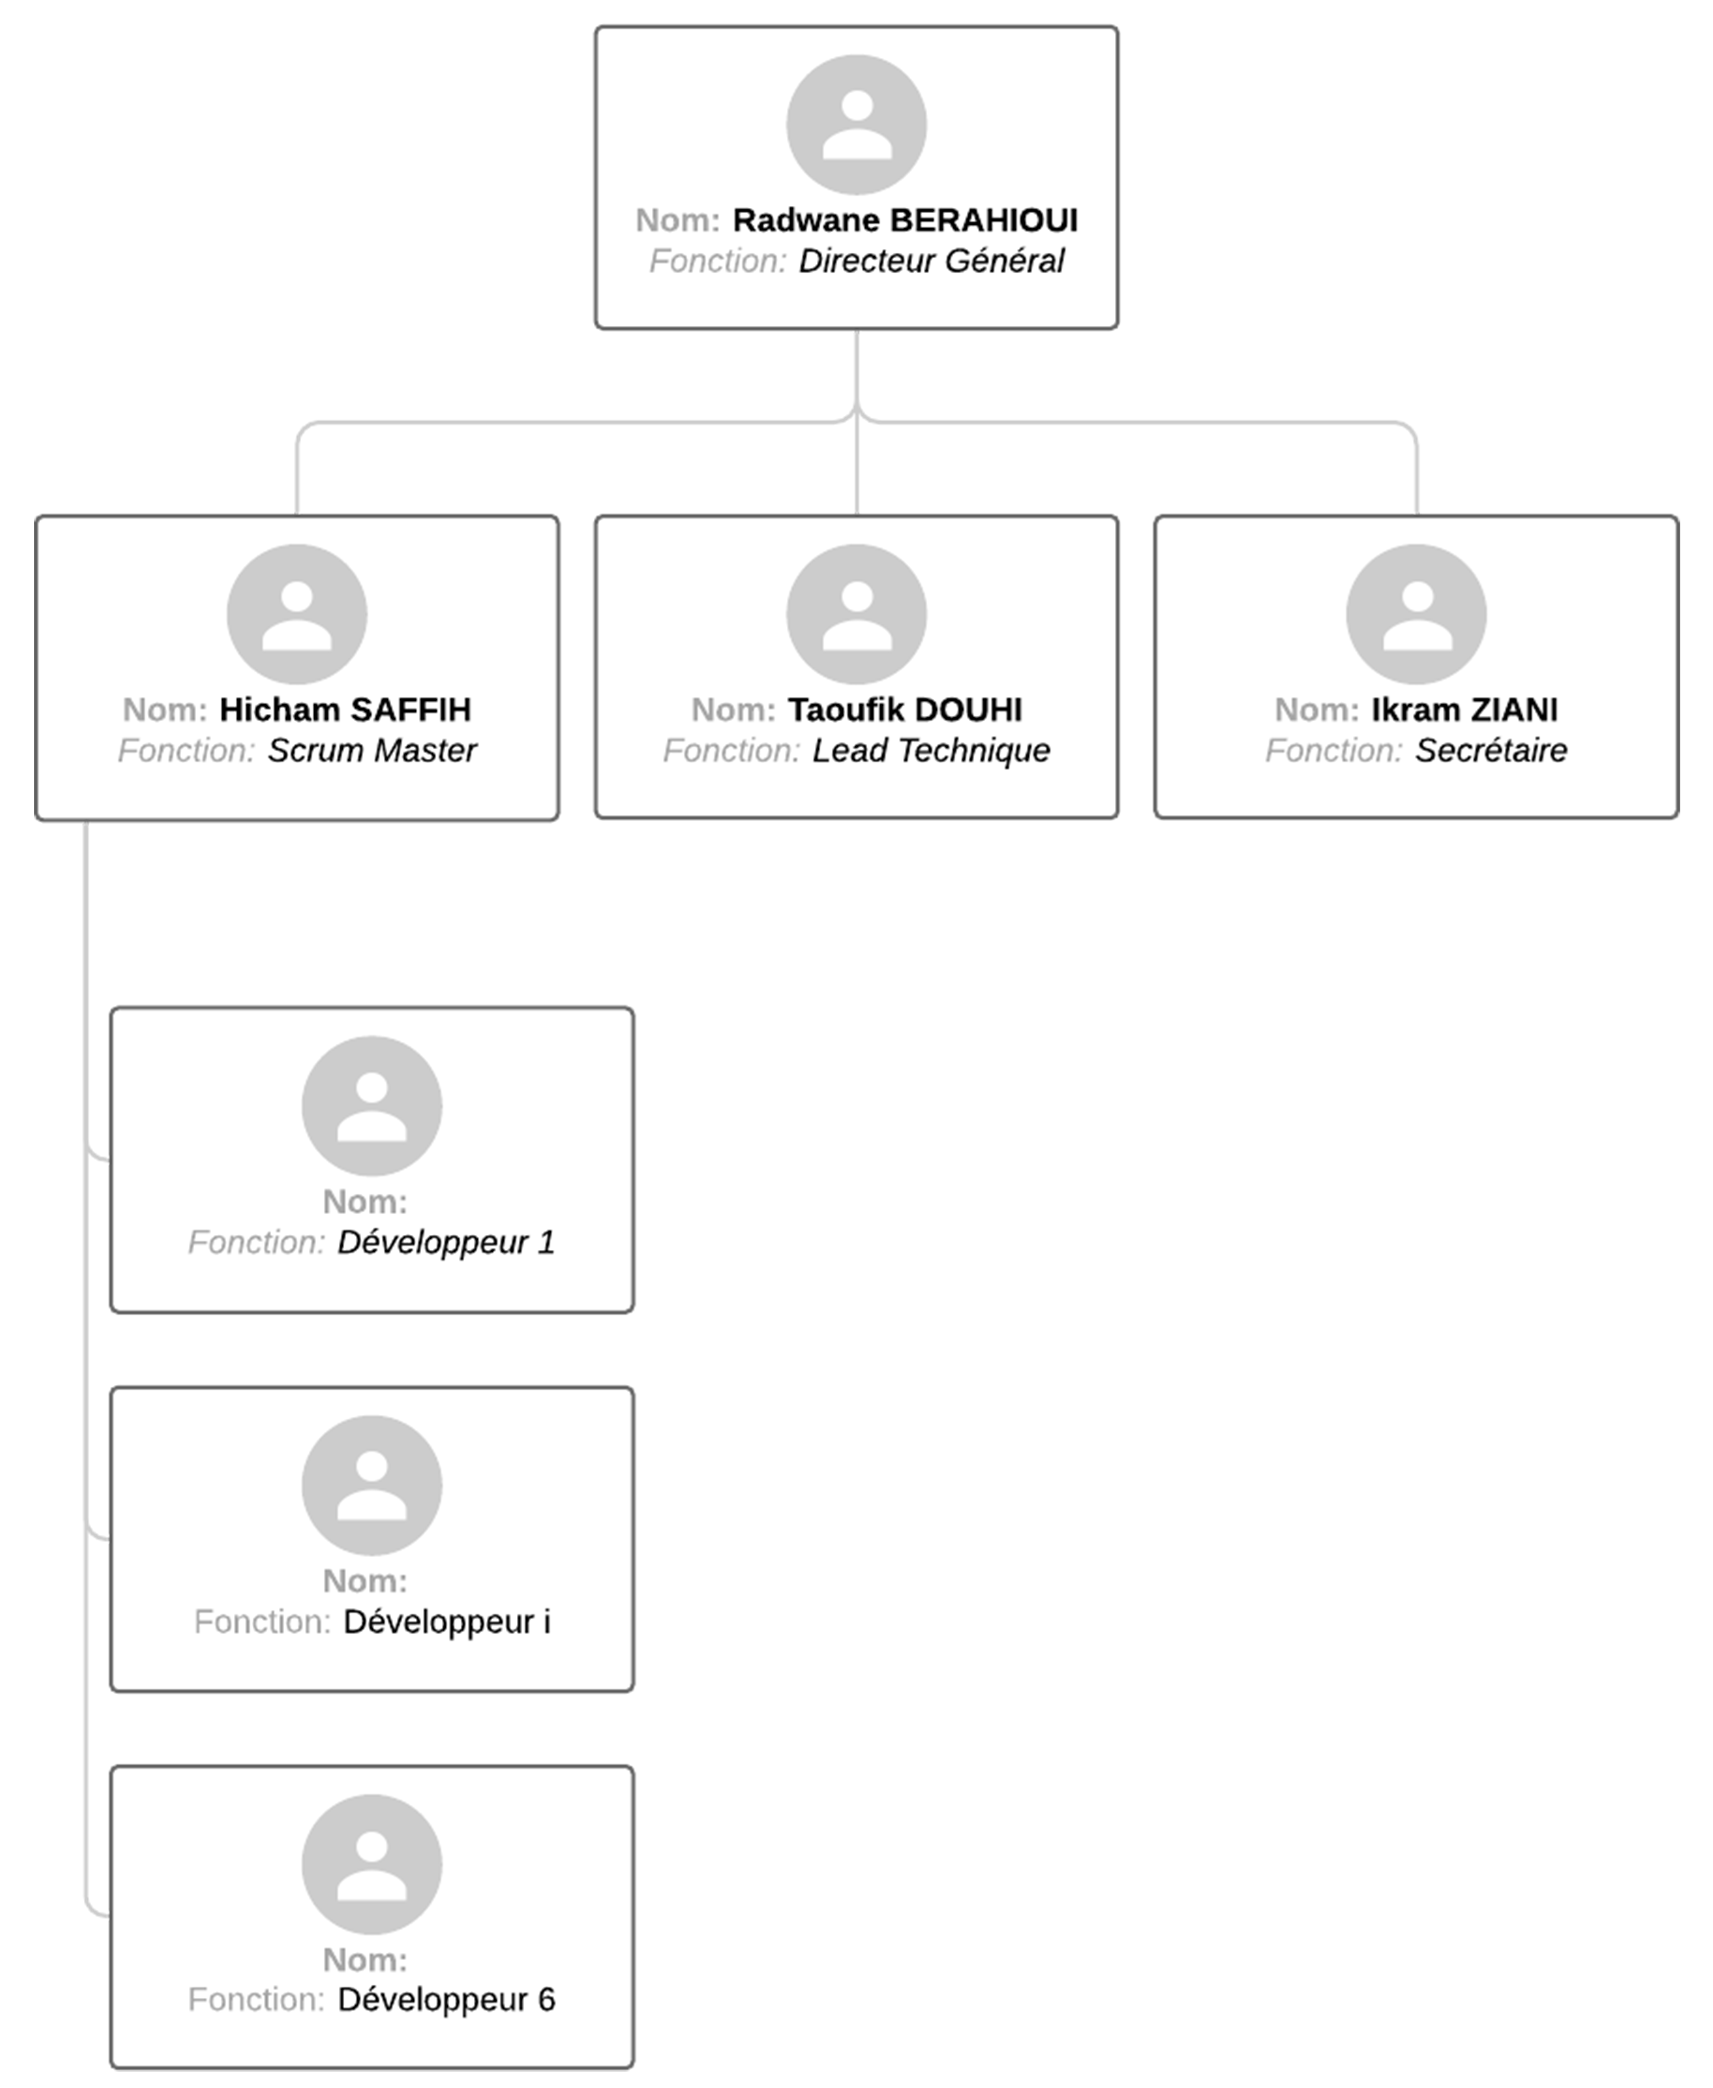
\includegraphics[width=1\textwidth]{algolus-organigramme.png}
		\caption{\textit{Organigramme de l'entreprise Algolus}}
		\label{fig:algolus-organigramme}
	\end{figure}
	
	\section{Description des besoins}
	
	\subsection{Problème}
	
	Dans le cadre du développement logiciel la détection et la correction des erreurs représentent un défi majeur, notamment en raison de la diversité des sources d’anomalies (logs, stack traces, captures d’écran, retours utilisateurs, etc.) et de la complexité croissante des applications. Les méthodes traditionnelles de débogage reposent souvent sur une analyse manuelle, ce qui est chronophage et sujet à des erreurs humaines. De plus, les solutions existantes peinent à offrir une approche générique et intelligente pour interpréter ces anomalies et proposer des correctifs pertinents.
	
	Ce défi prend une dimension particulière dans le cadre des activités de Algolus, la complexité des systèmes gérés par l'entreprise amplifie les difficultés de diagnostic des anomalies. Les équipes techniques consacrent actuellement un volume considérable de leurs ressources temporelles à l'analyse manuelle des incidents, retardant d'autant les mises en production. Par ailleurs, la variété des clients et des cas d'usage entraîne une hétérogénéité des remontées d'erreurs (rapports techniques détaillés pour les clients corporate vs. simples captures d'écran pour les utilisateurs finaux), ce qui rend inefficaces les outils de monitoring conventionnels utilisés jusqu'à présent. Ce constat a motivé l'entreprise à explorer des solutions d'IA générative capables d'unifier l'interprétation des anomalies.
	
	\subsection{Les besoins fonctionnels}
	
	Les besoins fonctionnels définissent les actions spécifiques que le système doit accomplir pour répondre aux exigences métier. Ils décrivent le "quoi", qu'est ce que le système doit faire, sous la forme de fonctionnalités concrètes de processus et d'interactions avec l'utilisateur. Ces exigences formulées par les parties prenantes  (les clients, les utilisateurs, et l'équipe produit) servent de base à la conception des cas d’usage et des scénarios de test.
	
	Pour garantir que le système de diagnostic d’erreurs réponde efficacement aux attentes des utilisateurs et des équipes techniques, nous avons identifié les besoins fonctionnels suivants :
	
	\begin{itemize}
		
		\item \textbf{Collecte et Pré-traitement des Données} : Extraction automatique des erreurs et des anomalies des systèmes à partir de :
		stacktraces, parsing des logs, captures d’écran, retours utilisateurs.
		
		\item \textbf{Analyse et Compréhension} : Analyse sémantique de retours d’erreurs, enrichissement contextuel : requêtage d’une base de connaissances (documentation technique, correctifs historiques).
		
		\item \textbf{Génération de Solutions} : Explication en langage naturel des causes racines, génération de correctifs (ex: snippets de code, étapes de résolution).
		
		\item \textbf{Interfaces utilisateurs} : Soumission des erreurs via des formulaires web pour uploader des stacktraces et des captures d'écran.
		
	\end{itemize}
	
	\subsection{Les besoins non fonctionnels}
	
	Les besoins non fonctionnels caractérisent le "comment", c'est à dire comment le système doit fonctionner, en précisant ses contraintes de qualité, de performance et d’infrastructure. Contrairement aux besoins fonctionnels, ils ne décrivent pas des fonctionnalités mais des critères tels que la rapidité, la sécurité, la scalabilité ou la facilité de maintenance. Leur respect est essentiel pour assurer la robustesse et l’efficacité du système en conditions réelles.
	
	Pour garantir une intégration harmonieuse dans l’écosystème existant et une expérience utilisateur optimale, les besoins non fonctionnels suivants ont été définies :
	
	\begin{itemize}
		
		\item \textbf{Performances} : Temps de réponse optimisé, et scalabilité : Support de plusieurs requêtes simultanées.
		
		\item \textbf{Intégration et Interopérabilité} : API REST, Endpoints standardisés et format de réponse avec schéma cohérent, support offline ; fonctionnement local avec Ollama.
		
		\item \textbf{Sécurité et Confidentialité} : Protection des données par chiffrement des échanges et anonymisation des logs utilisateurs (RGPD), et authentification : JWT pour l’accès aux APIs sensibles.	
		
		\item \textbf{Expérience Utilisateur} : Ergonomie, interface intuitive, Dark/Light mode et thèmes accessibles.
		
		
	\end{itemize}
	
	\subsection{Solutions envisagées}
	
	Ce projet vise à développer une application intelligente et modulaire permettant de détecter et de corriger automatiquement les anomalies logicielles, nous avons identifié les objectifs spécifiques suivants :
	
	\renewcommand{\labelitemi}{$\bullet$}
	\begin{itemize}
		\item Détecter avec un taux de réussite d'au moins 80\% les anomalies logicielles sur des sources multimodales.
		
		\item Proposer automatiquement des correctifs pertinents dans plus de 70\% des cas.
		
		\item Optimiser le temps moyen de résolution d’erreurs de 30\% par rapport aux méthodes manuelles.
	\end{itemize}
	
	Pour atteindre ces objectifs, nous avons envisagé une solution basée sur un ensemble de méthodes et technologies innovantes incluant :
	
	\begin{itemize}
		\item \textbf{Analyse Multimodale des Erreurs} : Implémenter un système capable d’interpréter des données hétérogènes (stack traces, logs texte, captures d’écran, etc.), et utiliser des techniques de RAG pour enrichir les requêtes avec une base de connaissances (code source, documentation technique, résolutions d’erreurs courantes).
		
		\item \textbf{Génération Automatique de Correctifs} : Exploiter des LLMs (via Ollama) pour suggérer des corrections précises et contextualisées.
		
		\item \textbf{Intégration et Scalabilité} : Développer un backend Spring Boot flexible, couplé à LangChain4j pour orchestrer les appels IA, et un système de gestion de base de données qui prend en charge les bases de données vectorielles, comme PostgeSQL, et permettre une extension future via des connecteurs pour différents outils de monitoring.
		
		\item \textbf{Optimisation et Évaluation} : mesurer l’efficacité du système via des métriques de précision (taux de détection, pertinence des correctifs), et effectuer un Benchmark : comparaison sur des jeux de données communs.
		
	\end{itemize}
	
	\section{Conclusion}
	
	En résumé, l’analyse initiale du problème nous a permis de cerner clairement les enjeux du projet et de définir des besoins fonctionnels et non fonctionnels cohérents avec les objectifs visés. L’étude des différentes solutions envisageables a conduit à des choix techniques adaptés, prenant en compte à la fois les contraintes de performance, d’ergonomie et de maintenabilité. Bien que certaines limitations persistent, notamment en lien avec l’évolutivité ou les dépendances externes, les bases posées offrent un cadre solide pour le développement et l’amélioration continue du système. Cette première partie dédiée à la définition du problème, des besoins, et des solutions envisagées, constitue une étape vers une solution complète, fiable et évolutive, et elle nous a permis de bien enchainer l'étape de l'analyse fonctionnelle et la conception du projet.
	
	\chapter{Analyse fonctionnelle et modélisation}
	
	\section{Introduction}
	
	Dans ce chapitre, nous mettons l'accent d'abord sur l'importance de l'analyse fonctionnelle en rappelons qu'est ce que c'est la modélisation UML, ses principes fondamentaux et son utilité dans le développement logiciel. Par la suite, nous exposerons les différents types de diagrammes utilisés dans notre étude, à savoir le diagramme de cas d’utilisation, et les diagrammes de séquences, après la définition de leurs composants.
	
	\section{Importance de l'analyse fonctionnelle}
	
	L’analyse fonctionnelle constitue une étape clé dans tous projets de développement informatique, car elle permet de bien comprendre les besoins du client et les contraintes du système à réaliser, identifier les fonctionnalités attendues, détecter les éventuelles incohérences et poser les bases d’une conception solide. De surcroit, une analyse fonctionnelle bien menée réduit considérablement les risques d’erreurs en phase de développement, facilite la planification du travail et améliore la qualité globale du produit final, ce qui lui rend essentielle pour assurer la réussite du projet.
	
	\section{Unified Modeling Language}
	
	Dans le cadre d’un projet de développement informatique la modélisation UML (Unified Modeling Language) joue un rôle essentiel en facilitant la compréhension, la conception et la communication autour du système à développer. UML propose un ensemble de diagrammes normalisés qui permettent de représenter visuellement les différentes dimensions d’un logiciel, telles que la structure, le comportement et les interactions entre les composants.
	
	L’utilisation des diagrammes UML comme les diagrammes de cas d’utilisation, de classes et de séquences permet de clarifier les besoins fonctionnels et non fonctionnels dès les premières phases du projet, de favoriser une meilleure communication entre les développeurs, les analystes et les clients, de surcroit il permet de détecter de façon précoce les incohérences ou erreurs potentielles dans la conception, et aussi de servir de documentation technique structurée pour le développement.
	
	Ainsi, UML constitue un outil précieux pour assurer la qualité, la cohérence et la pérennité d’un projet informatique, en apportant une vision globale et partagée du système.
	
	\section{Architecture hybride : LLM et RAG}
	
	Avant de présenter nos diagrammes de conception UML, il est nécessaire de définir leurs différents éléments composants. Voici une liste des éléments clés qui permettent au système de répondre aux besoins définies dans le chapitre précédent.
	
	\begin{itemize}
		
		\item \textbf{LLM (Large Language Model)} : Est un modèle d'intelligence artificielle pré-entraîné sur des volumes massifs de données textuelles, capable de comprendre, générer et manipuler le langage naturel de manière contextuelle. Il est basé sur des architectures de réseaux de neurones (comme les transformers), et excelle dans des tâches variées (réponse aux questions, traduction, synthèse de texte, etc.) en prédisant des séquences linguistiques d'une manière probabiliste. Contrairement aux systèmes traditionnels, un LLM ne suit pas de règles prédéfinies, mais apprend des motifs linguistiques en se basant sur des modèles non-supervisés.
		
		\item \textbf{RAG (Retrieval-Augmented Generation)} : Est une technique post-entrainement qui nous permet d'adapter l'usage des LLMs à travers l'enrichissement des réponses en recherchant des documents pertinents dans une base de connaissances externe, et en générant des réponses contextualisées à partir de ces sources. \cite{rag}
		Le RAG est composé de plusieurs éléments et services - dont nous allons parler tout de suite - organisés pour réaliser son objectifs.
		
		\item \textbf{Agent AI} : Une entité qui peut plannifier, exécuter des tâches d'une manière agentique ; Il reçoit les requêtes brutes de l'utilisateur, les enrichit en combinant plusieurs techniques avancées comme le RAG et la mémoire conversationnelle, puis les présente au modèle de langage sous une forme optimale.
		
		Parmi les atouts majeurs d'un Agent AI sa capacité de configurer d'une façon dynamique les trois parties constituant le prompt envoyé au LLM :
		
		\begin{itemize}
			
			\item \textbf{System Message} : définit le comportement global attendu du modèle (rôle, ton, contraintes, format de la réponse), en fixant un cadre pour l’interprétation des requêtes.
			
			\item \textbf{User Input} : correspond à la requête explicite formulée par l’utilisateur, exprimant son besoin ou sa question.
			
			\item \textbf{Few Shot Examples} : Quelques exemples de paires question/réponse (ou tâche/résultat), avant la question réelle de l’utilisateur, servant à orienter le comportement du modèle sans avoir à l'entraîner à nouveau.
			
		\end{itemize}
		
		\item \textbf{ChatModel} : Incarne le moteur de génération de langage naturel. Ce composant spécifique, configuré pour utiliser des modèles locaux ou externes, transforme les prompts structurés en analyses techniques détaillées.
		
		Le ChatModel permet de configurer plusieurs propriétés du LLM, citons les plus importantes :
		
		\begin{itemize}
			
			\item L'URL de base étant le point d'accès à l'API du modèle
			
			\item Le nom du modèle de langage à utiliser
			
			\item La Température, une propriété qui détermine le degré de créativité du LLM à formuler ses réponses, 0 étant le plus précis, et 1 le plus créatif.
			
			\item Le Timeout, qui est le délai maximal de réponse avant échéance.
			
		\end{itemize}
		
		\item \textbf{ChatMemory} : est un composant logiciel conçu pour conserver l’historique des échanges dans un système conversationnel (comme un chatbot), permettant ainsi de maintenir le contexte entre les messages et d’offrir des réponses plus cohérentes et personnalisées.
		
	\end{itemize}
	
	La liste ci-dessous met l'accent sur un élément particulier qui est le RAG, elle définie le rôle de chacun de ses composants :
	
	\begin{itemize}
		
		\item \textbf{Resource} : Constitue la matière première du système RAG. Il s'agit de la source originelle des données qui alimenteront la base de connaissances. Ces ressources peuvent prendre diverses formes : fichiers PDF contenant la documentation technique, pages web de référence, extraits de bases de données, ou tous autres supports contenant des informations pertinentes.
		
		\item \textbf{Tokenizer} : Joue un rôle fondamental dans le prétraitement du texte, il  décompose le contenu textuel en unités significatives appelées tokens, "un token peut correspondre à un mot entier, un sous-mot ou même un caractère individuel selon la méthode employée". Afin de rester dans les limites de longueur imposées par les modèles (souvent exprimées en nombre de tokens), le texte est ensuite segmenté en blocs appelés \textit{chunks}. Ces chunks sont de taille contrôlée (par exemple, 512 tokens), éventuellement avec un chevauchement partiel entre eux, pour ne pas perdre de contexte entre deux segments. Des algorithmes avancés comme ceux proposés par HuggingFace - une entreprise pionnière dans le domaine du traitement du langage naturel (NLP) et de l’intelligence artificielle - permettent une \textit{tokenisation} optimale qui préserve le sens tout en gérant les particularités linguistiques. La tokenisation joue un rôle cruciale car elle influe directement la qualité des embeddings générés ultérieurement.
		
		\item \textbf{DocumentParser} : Assure la transformation des ressources brutes en documents structurés, il comprend divers formats de fichiers (PDF, HTML, Markdown, etc.) et en extrait le contenu textuel significatif tout en conservant les métadonnées importantes. Des bibliothèques spécialisées comme sont souvent employées pour cette tâche complexe. Le DocumentParser nettoie également le texte en supprimant les éléments non pertinents (en-têtes, pieds de page, balises HTML) pour ne conserver que l'information essentielle.
		
		\item \textbf{Document} : Représente la forme normalisée et standardisée des informations après traitement. Chaque document contient non seulement le texte brut nettoyé, mais aussi des métadonnées descriptives (titre, auteur, date de création, source) qui faciliteront son identification et son utilisation ultérieure. Un identifiant unique est attribué à chaque document pour permettre son suivi tout au long du pipeline. Cette structuration rigoureuse est essentielle pour maintenir la cohérence des données dans les étapes suivantes du processus mené par le RAG.
		
		\item \textbf{EmbeddingModel} : Est au cœur de la transformation sémantique du système. Ce modèle sophistiqué convertit le texte en représentations vectorielles denses (embeddings) qui capturent le sens profond des contenus. Des modèles sont spécialisés dans cette tâche produisent des vecteurs où la similarité spatiale correspond à la similarité sémantique. La qualité de l'EmbeddingModel détermine directement la capacité du système à retrouver des documents pertinents pour une requête donnée.
		
		\item \textbf{EmbeddingStoreIngestor} : Orchestre le processus complet d'indexation des documents, il supervise plusieurs opérations critiques : il applique la tokenisation et la segmentation des textes, déclenche la génération des embeddings via l'EmbeddingModel, et gère le stockage final dans l'EmbeddingStore. \\ L'EmbeddingStoreIngestor implémente souvent des stratégies de traitement par lots pour optimiser les performances et peut gérer des pipelines complexes de prétraitement avant la vectorisation.
		
		\item \textbf{EmbeddingStore} : Sert de mémoire à long terme au système RAG, cette base de données vectorielle spécialisée stocke les embeddings générés et permet des recherches rapides de similarité. L'EmbeddingStore supporte des opérations massives d'insertion tout en maintenant des temps de réponse faibles pour les requêtes.
		
		\item \textbf{Retriever} : Est le composant qui établit le pont entre les questions des utilisateurs et la base de connaissances. Lors d'une requête, le Retriever sollicite de l'EmbeddingModel la transformation des questions des utilisateurs en embeddings, puis recherche dans l'EmbeddingStore les documents dont les vecteurs sont les plus proches. Ce composant implémente des algorithmes de similarité vectorielle (cosine similarity par exemple) et peut être finement paramétré (nombre de résultats retournés, seuil de similarité minimal). Le Retriever joue ainsi un rôle déterminant dans la pertinence des requêtes fournis au LLM.
		
	\end{itemize}
	
	Le diagramme montré dans la figure \ref{fig:diagramme-rag} synthétise d'une manière visuelle ces interactions.
	
	\begin{figure}[H]
		\centering
		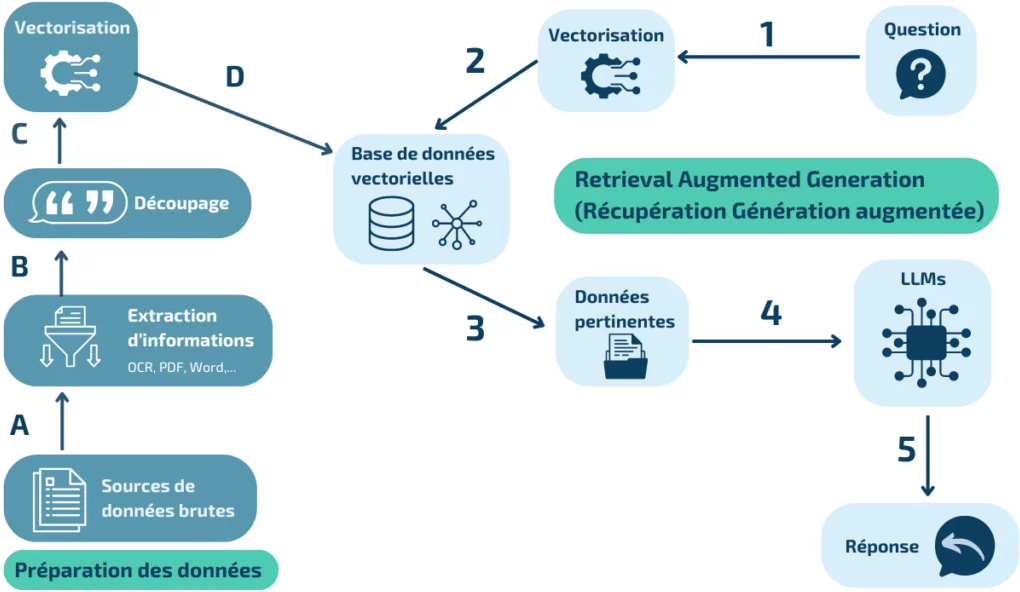
\includegraphics[width=1\textwidth]{diagramme-rag.png}
		\caption{\textit{Diagramme décrivant le fonctionnement d'un RAG}}
		\label{fig:diagramme-rag}
	\end{figure}
	
	\section{Diagramme de cas d'utilisation}
	
	Un diagramme de cas d'utilisation est une représentation visuelle des interactions entre les acteurs (utilisateurs, systèmes) et les fonctionnalités d'une application. Il identifie les besoins métiers sous forme d'actions (cas d’utilisation) et montre qui fait quoi, sans entrer dans les détails techniques.
	
	\subsection{Acteurs}
	
	Dans un diagramme de cas d'utilisation, les acteurs sont les entités qui interagissent avec le système pour accomplir un objectif précis. D'une part, un acteur peut être primaire (s'il est déclencheur d'un cas d'utilisation) ou secondaire (intervient dans un cas d'utilisation mais ne le déclenche pas), d'une autre part, un acteur peut être humain ou bien un acteur système.
	
	Dans notre cas, trois types d'acteurs sont impliqués  :
	
	\begin{itemize}
		\item \textbf{Utilisateur} : peut être un développeur ou un testeur qui rapporte une erreur, et peut interagir via une API REST ou bien une interface web.
		
		\item \textbf{Administrateur du système} : responsable de la mise à jour des connaissances du système et de la configuration des modèles.
		
		\item \textbf{Système} : le moteur de traitement intelligent, responsable d'analyser les anomalies, et de proposer des correctifs appropriés.
	\end{itemize}
	
	\subsection{Notre diagramme de cas d'utilisations}
	
	La figure \ref{fig:use-case} présente le diagramme de cas d'utilisation de notre application (voir la page 17).
	
	\begin{figure}[H]
		\centering
		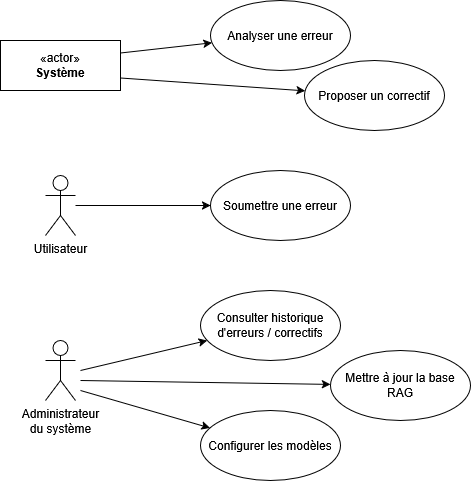
\includegraphics{use-case.drawio.png}
		\caption{\textit{Diagramme de cas d'utilisation}}
		\label{fig:use-case}
	\end{figure}
	
	\section{Description textuelle}
	
	La description du déroulement et les préconditions des actions pour chaque cas d'utilisation est une étape méticuleuse qui nécessite une grande réflexion. Nous commençons souvent par une première description basée sur les informations que nous obtenons.
	Généralement, une description textuelle comporte l'acteur principal (entité initiatrice), l'objectif (finalité métier), et les préconditions (conditions préalables de déclenchement). Le déroulement est ensuite décrit à travers deux scénarios complémentaires : le scénario nominal, qui présente la séquence optimale d'actions aboutissant au résultat attendu, et les scénarios alternatifs, qui couvrent les exceptions et parcours d'erreur.
	
	\textbf{Acteur Principal} : Utilisateur, développeur ou mainteneur logiciel confronté à une erreur technique ou fonctionnelle.	
	
	\textbf{Objectif} : Fournir un diagnostic précis et des correctifs pour des erreurs logicielles en combinant une description textuelle (stacktrace, logs), et une capture d'écran ou vidéo contextuelle.
	
	\textbf{Préconditions}
	
	\begin{itemize}
		\item Accès à l'interface web de l'application
		\item Services backend et modèle LLM (Ollama) opérationnels
		\item Base de connaissances locale (RAG) préchargée avec le code source pertinent
	\end{itemize}
	
	\textbf{Scénario Nominal}
	
	\begin{itemize}[label={}]
		\item \textbf{1. Soumission de la requête}
		\begin{itemize}
			\item Upload par l'utilisateur :
			\begin{itemize}
				\item Description textuelle de l'erreur
				\item Optionnellement une capture d'écran/vidéo
			\end{itemize}
			\item Envoi au contrôleur
		\end{itemize}
		
		\item \textbf{2. Traitement par l'Agent AI}
		\begin{itemize}
			\item Récupération du contexte via \texttt{chatMemory}
			\item Enrichissement via requête RAG :
			\begin{itemize}
				\item Extraction d'extraits de code pertinents
				\item Documents techniques liés
			\end{itemize}
		\end{itemize}
		
		\item \textbf{3. Appel au Modèle LLM}
		\begin{itemize}
			\item Formatage de la requête incluant :
			\begin{itemize}
				\item Description utilisateur
				\item Métadonnées multimédias
				\item Contexte historique + résultats RAG
			\end{itemize}
			\item Réponse structurée en 3 parties :
			\begin{verbatim}
				1 - Analyse de l'erreur : [diagnostic]
				2 - Source : [fichier:ligne]
				3 - Correctifs : [solutions]
			\end{verbatim}
		\end{itemize}
		
		\item \textbf{4. Post-Traitement}
		\begin{itemize}
			\item Sauvegarde dans \texttt{chatMemory}
			\item Journalisation de la transaction
		\end{itemize}
		
		\item \textbf{5. Affichage du résultat}
		\begin{itemize}
			\item Présentation claire avec mise en forme des chemins et snippets
		\end{itemize}
	\end{itemize}
	
	\textbf{Scénarios Alternatifs}
	
	\begin{description}
		\item{A1. Erreur sans capture d'écran}
		\begin{itemize}
			\item Ignore l'extraction visuelle
			\item Utilise uniquement texte et RAG
		\end{itemize}
		
		\item{A2. Échec du RAG }
		
		\begin{itemize}
			\item Utilise le contexte historique uniquement
			\item Journalise un avertissement
		\end{itemize}
		
		\item{A3. Timeout du LLM} 
		
		\begin{itemize}
			\item Nouvelle tentative après un délai
			\item Retourne message d'erreur clair
		\end{itemize}
	\end{description}
	
	\section{Diagrammes de séquences}
	
	Un diagramme de séquences est un type de diagramme UML utilisé pour modéliser les interactions entre les différents objets ou composants d'un système dans un scénario précis, il met en évidence l'ordre chronologique des messages échangés entre les acteurs et les objets, les interactions dynamiques entre les éléments du système, et la durée de vie des objets participant au scénario.
	
	Vu la complexité du système, et pour plus de visibilité, Nous avons élaboré deux diagrammes de séquences, un premier diagramme de séquences illustré dans la figure \ref{fig:ds-ai-agent} décrivant les interactions entre les entités générales, et un deuxième diagramme de séquences montré dans la figure \ref{fig:ds-rag.drawio} concentré sur les interactions au sein du RAG.
	
	\begin{figure}[H]
		\centering
		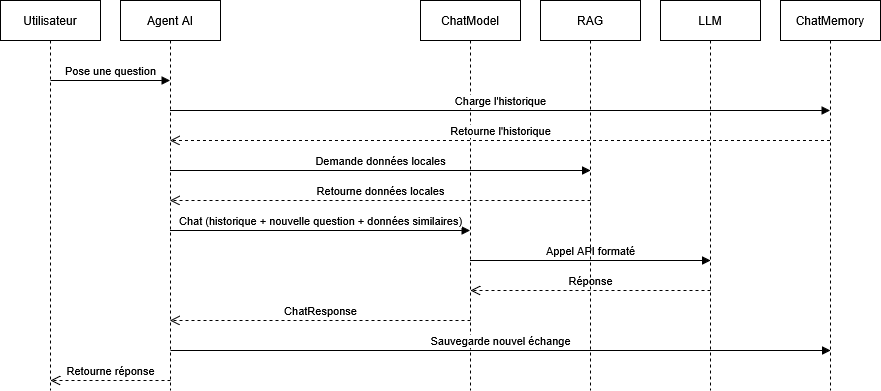
\includegraphics[width=1\textwidth]{ds-ai-agent.drawio.png}
		\caption{\textit{Diagramme de séquences décrivant le fonctionnement de l'agent AI}}
		\label{fig:ds-ai-agent}
	\end{figure}
	
	\begin{figure}[H]
		\centering
		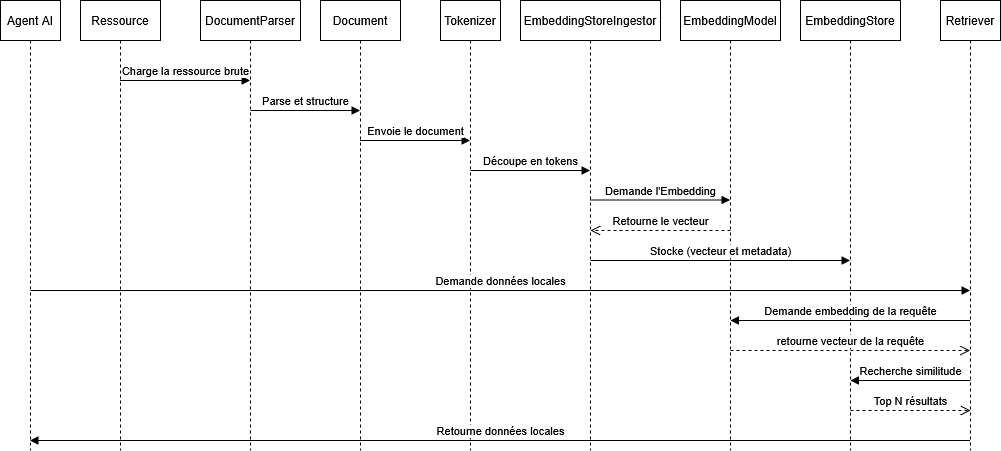
\includegraphics[width=1\textwidth]{ds-rag.drawio.png}
		\caption{\textit{Diagramme de séquences décrivant le fonctionnement d'un RAG}}
		\label{fig:ds-rag.drawio}
	\end{figure}
	
	\section{Conclusion}
	
	L’analyse fonctionnelle et la conception ont constitué des étapes fondamentales dans la structuration de notre projet. Les modèles et diagrammes produits ont servi de base solide pour la phase de développement, ils ont permis de formaliser les interactions entre les différents composants tout en anticipant d’éventuelles contraintes techniques.
	
	Enfin, cette phase préparatoire a mis en évidence l’importance d’une approche itérative, où l’analyse et la conception évoluent en parallèle des retours développeurs. Cette flexibilité méthodologique s’est avérée essentielle pour adapter le système aux besoins réels, tout en respectant les impératifs de qualité et de délais, ce qui sera constaté dans l'étape de réalisation.
	
	\chapter{Réalisation}
	
	\section{Introduction}
	
	Ayant mené à l'étude des dimensions fonctionnelles et techniques, nous abordons désormais l'étape cruciale de réalisation concrète du projet. Cette phase opérationnelle sera consacrée à l'implémentation effective de la solution.
	
	Ce chapitre présente la méthode de gestion adoptée, l'environnement de développement (outils, frameworks, librairies, etc.), l'architecture logicielle retenue et son adéquation avec les besoins, les défis techniques rencontrés et les solutions apportées, et les composants clés implémentés avec des extraits de code significatifs, et des captures d'écran illustrant les résultats obtenus.
	
	\section{Méthode de gestion adoptée : SCRUM}
	
	\subsection{Scrum à la théorie}
	
	Scrum est un cadre méthodologique agile destiné à optimiser la gestion de projets complexes, en particulier dans le domaine du développement logiciel. Il repose sur des itérations courtes appelées \textit{sprints}, au cours desquelles une équipe pluridisciplinaire s'engage à livrer un incrément fonctionnel du produit. Scrum définit des rôles précis (Scrum Master, Product Owner, équipe de développement), des artefacts (Product Backlog, Sprint Backlog, Increment) et des événements clés (Daily Scrum, Sprint Planning, Sprint Review, Sprint Retrospective). Sa structure vise à favoriser la transparence, l’inspection régulière du travail accompli et l’adaptation rapide face aux changements. En théorie, Scrum encourage une collaboration étroite, une communication continue et une amélioration itérative du produit et des processus.
	
	Les acteurs du framework SCRUM sont :
	
	\begin{itemize}
		
		\item \textbf{Product Owner} : Responsable de maximiser la valeur du produit en gérant le Product Backlog.
		
		\item \textbf{Scrum Master} : facilite le processus Scrum, veille à ce que l’équipe respecte le cadre et supprime les obstacles.
		
		\item \textbf{Équipe de développement} : équipe auto-organisée chargée de livrer un incrément du produit à la fin de chaque sprint.
		
	\end{itemize}
	
	La liste suivante définit brièvement les éléments clés de SCRUM :
	
	\begin{itemize}
		
		\item \textbf{Sprint} : itération fixe (généralement de 1 à 4 semaines) durant laquelle un incrément du produit est développé.
		
		\item \textbf{Product Backlog} : liste priorisée des fonctionnalités, exigences et corrections à apporter au produit.
		
		\item \textbf{Sprint Backlog} : sous-ensemble du \textit{Product Backlog} sélectionné pour être réalisé durant le sprint.
		
		\item \textbf{Increment} : résultat fonctionnel du sprint, potentiellement livrable et utilisable.
		
		\item \textbf{Sprint Planning} : réunion de planification en début de sprint pour définir les objectifs et les tâches à réaliser.
		
		\item \textbf{Daily Scrum} : réunion quotidienne courte (15 min) pour synchroniser l’équipe et adapter le plan de travail.
		
		\item \textbf{Sprint Review} : réunion de fin de sprint pour présenter l’incrément et recueillir des retours.
		
		\item \textbf{Sprint Retrospective} : réunion pour analyser le déroulement du sprint et identifier des pistes d’amélioration.
	\end{itemize}
	
	La figure \ref{fig:scrum} illustre comment un projet est géré avec la méthode SCRUM.
	
	\begin{figure}[H]
		\centering
		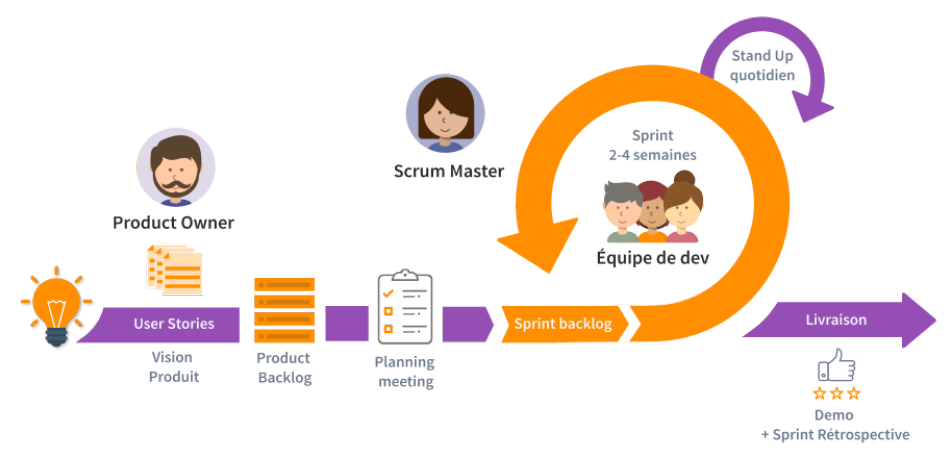
\includegraphics[width=1\textwidth]{scrum.png}
		\caption{\textit{Gestion de projet avec SCRUM}}
		\label{fig:scrum}
	\end{figure}
	
	\subsection{Scrum à la pratique}
	
	\subsubsection{Equipe du projet}
	
	\begin{table}[H]
		\centering
		\caption{\textit{Tableau des acteurs SCRUM}}
		\begin{tabular}{|l|l|}
			\hline
			\textbf{Rôle} & \textbf{Acteur} \\
			\hline
			Product Owner & BERAHIOUI Radwane \\
			\hline
			SCRUM Master & BERAHIOUI Radwane \\
			\hline
			Developpers & LOUDIYI Hicham \\
			\hline
			Tech Lead & BERAHIOUI Radwane \\
			\hline
		\end{tabular}
		\label{tab:equipe-projet}
	\end{table}
	
	\subsubsection{Sprints du projet}
	
	Pour la planification du projet, nous utilisons l’outil de messagerie collaborative Slack. Il joue un rôle central dans la communication entre le Tech Lead et le développeur, tout en offrant une visibilité claire sur l’avancement global du projet. Slack facilite le suivi des sprints, la coordination des tâches et la gestion des différentes étapes du développement. Grâce à ses fonctionnalités de planification et de suivi, il contribue à une organisation efficace et structurée du travail en équipe.
	
	\section{Stack technique}
	
	\subsection{Langages}
	
	\subsubsection{Java}
	
	\begin{figure}[H]
		\begin{minipage}{0.8\textwidth}
			Java est un langage de programmation orienté objet, robuste et multiplateforme, largement utilisé dans le développement d'applications d'entreprise. Sa forte typographie, sa gestion automatique de la mémoire (via le garbage collector) et son écosystème riche (bibliothèques, frameworks) en font un choix idéal pour les systèmes backend complexes. la version utilisée est Java 17.
		\end{minipage}
		\hfill
		\begin{minipage}{0.15\textwidth}
			\begin{figure}[H]
				\centering
				
\includegraphics[width=\linewidth]{java-logo.png}
				\label{fig:java-logo}
			\end{figure}			
		\end{minipage}
	\end{figure}
	
	\subsection{Frameworks}
	
	\subsubsection{Spring}
	
	\begin{figure}[H]
		\begin{minipage}{0.8\textwidth}
			Spring est un framework modulaire pour Java, simplifiant le développement d'applications grâce à l’inversion de contrôle (IoC) et la programmation orientée aspect (AOP). La version utilisée est 6.1.8.
		\end{minipage}
		\hfill
		\begin{minipage}{0.15\textwidth} 
			\begin{figure}[H]
				\centering
				
\includegraphics[width=\linewidth]{spring-logo.png}
				\label{fig:spring-logo}
			\end{figure}
		\end{minipage}
	\end{figure}
	
	\subsubsection{Spring Boot}
	
	\begin{figure}[H]
		\begin{minipage}{0.8\textwidth}
			Spring Boot étend Spring en fournissant des configurations automatiques, un serveur embarqué (Tomcat, Netty) et des outils clés en main (Spring Data, Spring Security), permettant de créer des applications standalone rapidement. La version utilisée est 3.4.5.
		\end{minipage}
		\hfill
		\begin{minipage}{0.15\textwidth} 
			\begin{figure}[H]
				\centering
				
\includegraphics[width=\linewidth]{spring-boot-logo.png}
				\label{fig:spring-boot-logo}
			\end{figure}
		\end{minipage}
	\end{figure}
	
	
	\subsubsection{LangChain4j}
	
	\begin{figure}[H]
		\begin{minipage}{0.8\textwidth}
			LangChain4J est une bibliothèque Java inspirée de LangChain (Python), conçue pour intégrer facilement des LLMs (Modèles de Langage) dans des applications. Elle offre des abstractions pour la gestion des prompts, le RAG, les appels aux modèles (OpenAI, Ollama, etc.), et la connexion à des bases de données vectorielles. La version utilisée est 1.0.0-alpha1.
		\end{minipage}
		\hfill
		\begin{minipage}{0.15\textwidth} 
			\begin{figure}[H]
				\centering
				
\includegraphics[width=\linewidth]{langchain4j-logo.png}
				\label{fig:langchain4j-logo}
			\end{figure}
		\end{minipage}
	\end{figure}
	
	\subsection{Bibliothèques}
	
	\subsubsection{Apache Commons}
	
	\begin{figure}[H]
		\begin{minipage}{0.8\textwidth}
			Apache Commons est une bibliothèque Java open-source fournissant des composants réutilisables pour simplifier le développement. Dans ce projet, elle sert à combler des besoins techniques récurrents avec des solutions optimisées et robustes. La version utilisée est 3.14.0.
		\end{minipage}
		\hfill
		\begin{minipage}{0.15\textwidth} 
			\begin{figure}[H]
				\centering
				
\includegraphics[width=\linewidth]{apache-commons-logo.png}
				\label{fig:apache-commons-logo}
			\end{figure}
		\end{minipage}
	\end{figure}
	
	\subsection{Systèmes de gestion de bases de données}
	
	\subsubsection{PostgreSQL}
	
	\begin{figure}[H]
		\begin{minipage}{0.8\textwidth}
			PostgreSQL est un système de gestion de base de données relationnelle (SGBDR) open-source, robuste et extensible. Dans le cadre de ce projet, il joue un rôle central pour stocker et gérer les données structurées nécessaires au bon fonctionnement de l’application, et fournit des plugins pour l'IA, notamment PgVector, qui gère les bases de données vectorielles. La version utilisée est 16.3
		\end{minipage}
		\hfill
		\begin{minipage}{0.15\textwidth} 
			\begin{figure}[H]
				\centering
				
\includegraphics[width=\linewidth]{postgresql-logo.png}
				\label{fig:postgresql-logo}
			\end{figure}
		\end{minipage}
	\end{figure}
	
	\subsection{Outils et environnement}
	
	\subsubsection{Ollama}
	
	\begin{figure}[H]
		\begin{minipage}{0.8\textwidth}
			Ollama est un outil open-source permettant d’exécuter localement des LLMs (comme Llama 3, Mistral, Gemma) sans dépendre d’une API externe. Il est idéal pour prototyper des solutions IA offline, contrôler les coûts et la confidentialité des données, et personnaliser finement les modèles via des modelfiles. [2]
			
			La version utilisée est 0.9.2
		\end{minipage}
		\hfill
		\begin{minipage}{0.15\textwidth} 
			\begin{figure}[H]
				\centering
				
\includegraphics[width=\linewidth]{ollama-logo.png}
				\label{fig:ollama-logo}
			\end{figure}
		\end{minipage}
	\end{figure}
	
	\subsubsection{Maven}
	
	\begin{figure}[H]
		\begin{minipage}{0.8\textwidth}
			Outil de build automatisé pour projets Java, qui gère Les dépendances (téléchargement auto), le packaging (JAR/WAR), et les cycles de compilation/test. La version utilisée est 3.9.10
		\end{minipage}
		\hfill
		\begin{minipage}{0.15\textwidth} 
			\begin{figure}[H]
				\centering
				
\includegraphics[width=\linewidth]{maven-logo.png}
				\label{fig:maven-logo}
			\end{figure}
		\end{minipage}
	\end{figure}
	
	\subsubsection{IntelliJ IDEA}
	
	\begin{figure}[H]
		\begin{minipage}{0.8\textwidth}
			IntelliJ IDEA est un IDE puissant pour Java/Kotlin, développé par JetBrains. Ses avantages incluent une analyse intelligente du code (suggestions, détection d’erreurs), une intégration native avec Spring Boot et Maven/Gradle, des outils pour le débogage, le profiling et les tests, et des extensions pour l’IA (ex : GitHub Copilot). La version utilisée est 2025.1 (Ultimate Edition)
		\end{minipage}
		\hfill
		\begin{minipage}{0.15\textwidth} 
			\begin{figure}[H]
				\centering
				
\includegraphics[width=\linewidth]{intellij-logo.png}
				\label{fig:intellij-logo}
			\end{figure}
		\end{minipage}
	\end{figure}
	
	\subsubsection{Git}
	
	\begin{figure}[H]
		\begin{minipage}{0.8\textwidth}
			Git est un système de contrôle de version distribué, essentiel pour le développement collaboratif. Il permet de suivre les modifications du code source, de gérer les branches, et de fusionner les travaux de plusieurs contributeurs. Grâce à des plateformes comme GitHub, il facilite le partage et la revue de code. Son utilisation améliore la traçabilité, la qualité et la productivité dans les projets logiciels. La version utilisée est 2.47.1.windows.2.
		\end{minipage}
		\hfill
		\begin{minipage}{0.15\textwidth} 
			\begin{figure}[H]
				\centering
				
\includegraphics[width=\linewidth]{git-logo.png}
				\label{fig:git-logo}
			\end{figure}
		\end{minipage}
	\end{figure}
	
	\section{Architecture technique du projet}
	
	Le projet repose sur une architecture modulaire et évolutive, construite autour des meilleures pratiques du développement Java moderne, de l'IA générative et de l’ingénierie logicielle. Il s’appuie sur les technologies suivantes :
	
	\begin{itemize}
		
		\item \textbf{Spring Boot} : Est le framework retenu pour le développement de la couche back-end. Il s’agit d’un choix stratégique largement justifié par les besoins du projet en termes de performance, de maintenabilité et d’intégration avec des composants d’intelligence artificielle.
		
		Spring Boot permet de structurer l’application de manière modulaire, en séparant clairement les responsabilités (contrôleurs, services, configuration, etc.). Cette organisation favorise une bonne lisibilité du code et facilite son évolution.
		
		L’application est également portable, dans la mesure où elle peut être conditionnée sous forme de JAR exécutable et déployée facilement sur tout environnement compatible Java, sans dépendance à un serveur externe.
		
		Un autre atout majeur est le caractère évolutif de Spring Boot : il s’intègre naturellement avec des bibliothèques telles que LangChain4j ou des bases de données comme PostgreSQL, ce qui permet d’ajouter de nouvelles fonctionnalités (IA, recherche vectorielle, mémoire contextuelle) sans remise en cause de l’existant.
		
		Le framework est aussi testable : il propose des outils natifs pour la réalisation de tests unitaires et d’intégration, garantissant la qualité et la stabilité du code produit.
		
		Enfin, Spring Boot est hautement extensible, alors si le projet venait à croître en complexité, il serait tout à fait envisageable de faire évoluer l’architecture vers un modèle microservices avec des outils comme Spring Cloud.
		
		\item \textbf{LangChain4j} : Pour permettre l’analyse intelligente des erreurs à l’aide d’un modèle de langage (LLM), le projet s’appuie sur la bibliothèque LangChain4j, une adaptation Java du framework LangChain initialement développé pour Python. Ce composant joue un rôle central dans l’intégration des fonctionnalités d’intelligence artificielle générative.
		
		LangChain4j facilite la mise en œuvre d’un mécanisme de RAG (Retrieval-Augmented Generation), en combinant génération de texte via un LLM et récupération de documents pertinents à partir d’une base vectorielle. Il s’intègre naturellement avec un modèles de langage, et avec des composants tels que la mémoire de conversation, le modèle d’embedding et le store d’embeddings.
		
		L’utilisation de LangChain4j rend l’application extensible et modulaire, car ses composants (LLM, mémoire, embeddings, etc.) sont interchangeables via des interfaces. Elle offre également un haut niveau de configurabilité, permettant d’adapter dynamiquement les modèles utilisés, la taille de la mémoire contextuelle ou encore les critères de pertinence documentaire.
		
		Enfin, son intégration avec Spring Boot via des beans injectables simplifie grandement sa mise en œuvre dans l’architecture globale du projet. Cela permet d’enrichir les traitements métier avec une couche d’IA tout en conservant la lisibilité et la testabilité du code.
		
		\item \textbf{Ollama} : Pour exécuter les modèles de langage en local sans dépendre de services cloud externes, le projet intègre Ollama, une plateforme légère permettant de servir des LLM open-source tels que Mistral, Llama3 ou Qwen qui offre des versions multimodales. Ollama agit comme un point d’accès HTTP local à un modèle de génération de texte, que LangChain4j peut interroger de manière transparente.
		
		Ce choix présente plusieurs avantages : tout d’abord, il rend l’application autonome et portable, car aucun appel à une API cloud (comme OpenAI ou Hugging Face) n’est requis. Cela permet un déploiement sur des machines locales ou en environnement isolé (on-premise), tout en respectant les contraintes de confidentialité des données.
		
		Grâce à une configuration centralisée (adresse du serveur, modèle utilisé, température, etc.), Ollama est également hautement configurable. Son intégration dans le projet se fait via des beans Spring instanciés dynamiquement dans la classe de configuration (AiConfig), ce qui permet d’adapter ou changer le modèle utilisé sans modifier la logique métier.
		
		Enfin, en travaillant de concert avec LangChain4j, Ollama permet la génération de réponses contextualisées et pertinentes, en tenant compte des documents récupérés et des interactions passées. Cela renforce la capacité de l'application à fournir des analyses d'erreurs enrichies, précises et directement exploitables.
		
		\item \textbf{PostgreSQL} : Utilisé comme système de gestion de base de données relationnelle, avec une orientation spécifique vers le stockage vectoriel, dans le cadre de l’indexation et de la recherche de documents sémantiques. Grâce à l’extension pgvector, PostgreSQL devient capable de stocker des vecteurs d’embedding et d’effectuer des recherches de similarité, essentielles dans une approche RAG (Retrieval-Augmented Generation).
		
		Le choix de PostgreSQL repose sur plusieurs critères clés : sa fiabilité, sa scalabilité et sa maturité en production. En plus de gérer des données relationnelles classiques (logs, utilisateurs, paramètres…), il peut aussi indexer efficacement des vecteurs issus des modèles d’embedding, et permettre des requêtes de type nearest neighbor search.
		
		Son intégration avec Spring Boot est fluide grâce à JPA ou JDBC, et son usage dans ce projet est évolutif : dans un premier temps, les embeddings sont stockés en mémoire (InMemoryEmbeddingStore), mais la bascule vers PostgreSQL permettra une persistance et une scalabilité bien supérieures, tout en conservant une interface compatible avec les composants LangChain4j.
		
		Ainsi, PostgreSQL joue un rôle fondamental dans la stratégie d’enrichissement contextuel des requêtes utilisateur, en permettant à l’IA de s’appuyer sur des documents pertinents stockés localement de façon fiable et interrogeable.
		
	\end{itemize}
	
	\begin{figure}[H]
		\centering
		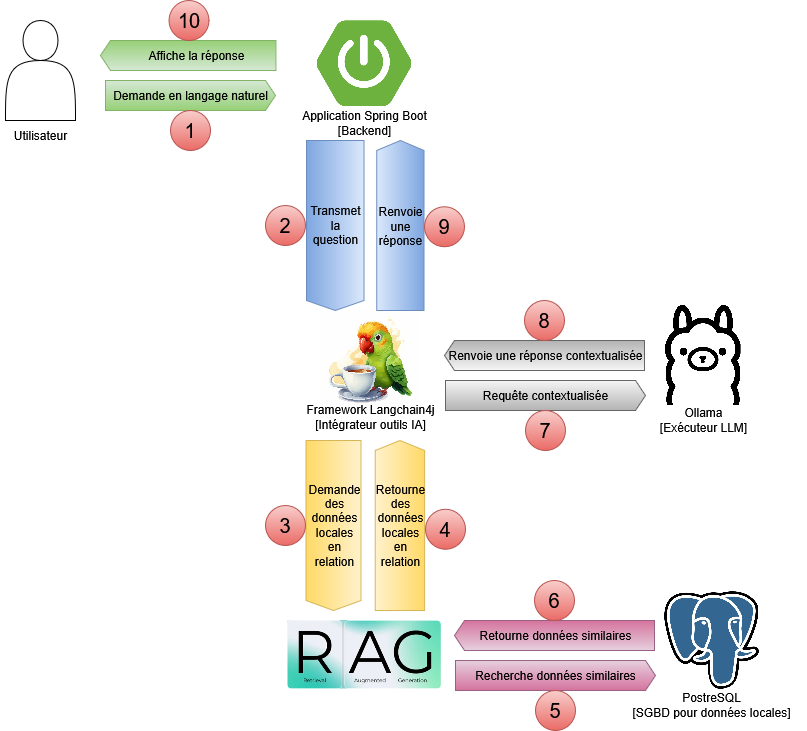
\includegraphics[width=1\textwidth]{illustration-graphique.drawio.png}
		\caption{\textit{Diagramme d'architecture technique}}
		\label{fig:illustration-graphique}
	\end{figure}
	
	La figure \ref{fig:illustration-graphique} illustre de manière synthétique les interactions entre les principaux composants techniques de l’architecture mise en place dans le cadre de ce projet. L'enchainement commence par la soumission d'une requête par un utilisateur, le backend Spring Boot reçois cette requête et la délègue au framework LangChain4j, ce dernier sollicite du RAG - qui aura déjà chargé sa base de connaissances dans une base de données vectorielle - des données en relation avec la requête, puis encapsule ces données avec la requête et l'historique de conversation pour envoyer cet ensemble à Ollama, qui à son tour communique avec le LLM et reçoit une réponse, qui finit par arriver à l'utilisateur.
	
	\section{Bonnes pratiques appliquées du développement Java}
	
	Dans le développement logiciel, l'adoption de bonnes pratiques de codage est essentielle pour garantir la robustesse, la maintenabilité et l'évolutivité des applications. Un code bien structuré, avec une logique claire et une réduction des redondances, facilite non seulement les futures modifications, mais améliore aussi la collaboration entre développeurs. Cette section aborde des principes clés que nous avons suivis pour optimiser l'écriture du code, en mettant l'accent sur les méthodes que nous avons appliquées pour améliorer la qualité tout en réduisant les risques d'erreurs.
	
	\subsection{L'importance d'une nomenclature claire et cohérente}
	
	Une nomination précise des classes et méthodes est essentielle pour garantir la maintenabilité et la lisibilité du code. Dans notre projet, nous avons porté une attention particulière aux noms de classes, d'attributs et de méthodes, afin de permettre à un lecteur de code de comprendre immédiatement le rôle de chaque composant sans avoir à explorer son implémentation.
	
	Citons quelques exemples concrets dans notre projet, la classe \verb|ErrorAnalysisService| indique clairement qu'elle orchestre la logique métier de l'analyse d'erreurs, tandis que \verb|FileValidator| évoque sans ambiguïté sa responsabilité : valider les fichiers entrants. De même, les méthodes comme \verb|extractKeyFrames()| (dans \verb|VideoProcessor|) ou \\ \verb|analyzeErrorWithRag()| (dans \verb|ErrorAnalysisAgent|) décrivent explicitement leurs actions et leurs spécificités techniques. À l'inverse, des noms vagues comme \verb|process()| ou \verb|handle()| auraient rendu le code obscur, obligeant les développeurs à parcourir le code source pour en comprendre la finalité. Par cette rigueur lexicale nous avons facilité aussi la collaboration entre équipes en réduisant les risques d'erreurs lors des évolutions futures. En résumé, un bon nommage agit comme une documentation intrinsèque, reflétant directement l’intention de conception et les principes métiers sous-jacents.
	
	\subsection{Utilisation de Bibliothèques Matures : Apache Commons}
	
	Plutôt que de réinventer la roue, nous avons utilisé des bibliothèques robustes comme Apache Commons, qui fournit des utilitaires optimisés pour plusieurs opérations telles que la manipulation de collections, les opérations sur les chaînes, et les validations.
	
	Pour mettre en lumière les utilisations de ces utilitaires dans notre projet, prenons par exemple la méthode \verb|estimateTokenCountInText(String text)| de la classe \\ \verb|TokenizerMyAppImpl|, dont la figure \ref{fig:before-string-utils} montre une implémentation classique, utilisant l'instruction de branchement conditionnel \verb|if| couplée aux opérateurs logiques.
	
	\begin{figure}[H]
		\centering
		\fbox{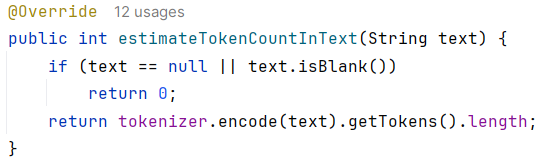
\includegraphics{before-string-utils.png}}
		\caption{\textit{Implémentation sans utiliser Apache Commons}}
		\label{fig:before-string-utils}
	\end{figure}
	
	Cette approche, bien que fonctionnelle, présente plusieurs limitations : la combinaison de deux vérifications dans une même condition, la duplication de cette logique à de nombreux endroits du code, et le risque potentiel de \verb|NullPointerException|.
	
	L'adoption d'une nouvelle implémentation exploitant la bibliothèque Apache Commons est montrée dans la figure \ref{fig:after-string-utils}.
	
	\begin{figure}[H]
		\centering
		\fbox{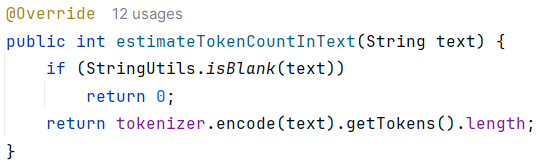
\includegraphics{after-string-utils.png}}
		\caption{\textit{Implémentation en utilisant Apache Commons}}
		\label{fig:after-string-utils}
	\end{figure}
	
	La méthode \verb|isBlank()| de la classe \verb|StringUtils| retourne \verb|true| dans trois cas : si \verb|text| est \verb|null|, ou une chaine de caractères vides, ou une chaine de caractères ne contenant que des espaces blancs, Ce qui donne plus de robustesse au projet, en évitant les \verb|NullPointerException| sans besoin de vérifier null explicitement, améliore la lisibilité en remplaçant une condition complexe par un seul appel clair, et garantit un comportement uniforme dans tout le projet.
	
	\subsection{Approches de parcours de collections en Java}
	
	Durant le développement, nous avons été amené à manipuler des collections de données. Plusieurs approches s'offraient alors à nous, chacune présentant des caractéristiques distinctes :
	
	\begin{itemize}
		
		\item \textbf{La boucle for traditionnelle} : Parcours indexé idéal pour les listes et tableaux, offrant un contrôle précis des positions mais inadapté aux collections non ordonnées comme les \verb|Set|.
		
		\item \textbf{La boucle for-each} : Introduite dans Java 5, c'est une syntaxe simplifiée pour itérer sur tous les éléments d'une collection, évitant les erreurs d'index mais interdisant les modifications pendant le parcours.
		
		\item \textbf{L'Iterator} : Permet un parcours séquentiel avec suppression sécurisée via \verb|remove()|, compatible avec toutes les collections mais plus verbeux à écrire.
		
		\item \textbf{Les Streams} : Approche déclarative exploitant des opérations fonctionnelles (filtrage, mapping) pour un code lisible et chainable, optimisé pour les traitements de données. [3]
		
		\item \textbf{ParallelStream} : Version parallélisée des Streams utilisant plusieurs cœurs CPU pour accélérer le traitement des gros volumes de données, au prix d'une complexité accrue en synchronisation.
		
	\end{itemize}
	
	Pour faire le bon choix, le tableau \ref{tab:parcours_collections} donne une comparaison entre ces approches selon différents critères.
	
	\begin{table}[H]
		\centering
		\caption{\textit{Comparaison des méthodes de parcours de collections en Java}}
		\label{tab:parcours_collections}
		\resizebox{\textwidth}{!}{ % Redimensionne le tableau
			\begin{tabular}{|>{\raggedright\arraybackslash}p{2.6cm}|c|c|c|c|c|}
				\hline
				\textbf{Critère} & 
				\textbf{\texttt{for}} & 
				\textbf{\texttt{for-each}} & 
				\textbf{\texttt{Iterator}} & 
				\textbf{\texttt{Stream}} & 
				\textbf{\texttt{ParallelStream}} \\
				\hline
				
				Modification possible & Risqué & Interdit & \texttt{remove()} & Interdit & Interdit \\
				\hline
				
				Accès par index & Oui & Non & Non & Non & Non \\
				\hline
				
				Lisibilité & Moyenne & Bonne & Faible & \makecell{Excellente\\(déclaratif)} & \makecell{Excellente\\(déclaratif)} \\
				\hline
				
				Types de sources & \makecell{List/\\Array} & \texttt{Iterable} & \texttt{Collection} & \makecell{Collection,\\Array, flux, etc.} & \makecell{Collection,\\Array, flux, etc.} \\
				\hline
				
				Performance & Optimale & \makecell{Légère\\baisse} & \makecell{Légère\\baisse} & \makecell{Bonne\\(selon cas)} & \makecell{Variable\\(multi-thread)} \\
				\hline
				
				Opérations intégrées & Non & Non & Non & Oui & Oui \\
				\hline
				
				Parallélisme & Difficile & Impossible & Impossible & Possible & \makecell{Automatique\\(Fork/Join)} \\
				\hline
				
				Gestion du \texttt{null} & Manuel & Manuel & Manuel & \texttt{Optional} & \texttt{Optional} \\
				\hline
				
				Cas d’usage typique & \makecell{Parcours indexé} & \makecell{Parcours simple\\séquentiel} & \makecell{Suppression\\d’éléments} & \makecell{Traitement\\fonctionnel} & \makecell{Traitement\\parallèle intensif} \\
				\hline
			\end{tabular}
		}
	\end{table}
	
	Prenons un exemple de notre projet, dans une implémentation de l'interface \verb|Tokenizer| fournie par LangChain4j, la méthode \\ \verb|estimateTokenCountInTools(Iterable<Object> objectsWithTools)| a été implémentée dans un premier temps en utilisant une boucle \verb|foreach|, comme le montre la figure \ref{fig:before-stream}.
	
	\begin{figure}[H]
		\centering
		\fbox{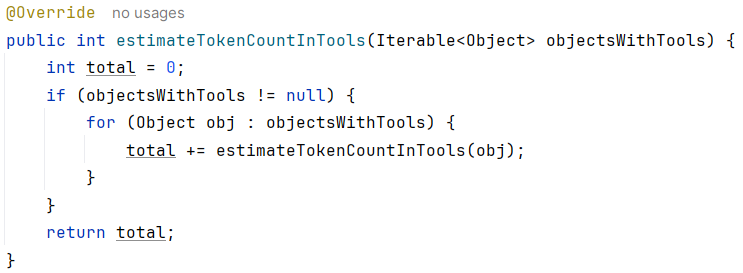
\includegraphics{before-stream.png}}
		\caption{\textit{Implémentation sans utiliser les Streams}}
		\label{fig:before-stream}
	\end{figure}
	
	Une évolution de cette implémentation utilisant les Streams ainsi que la bibliothèque Apache Commons est illustrée dans la figure \ref{fig:after-stream}.
	
	\begin{figure}[H]
		\centering
		\fbox{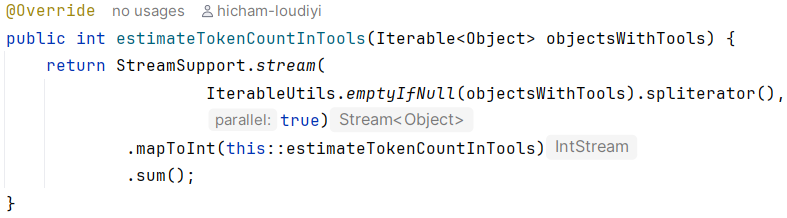
\includegraphics[width=1\textwidth]{after-stream.png}}
		\caption{\textit{Implémentation en utilisant les Streams}}
		\label{fig:after-stream}
	\end{figure}
	
	Cette implémentation, offrant une gestion robuste des null avec \\ \verb|IterableUtils.emptyIfNull()|, convertit l'Iterable en Stream parallélisable avec \\ \verb|StreamSupport.stream(..., true)|, ce qui permet un traitement réparti sur plusieurs cœurs CPU si la collection est grande, et une optimisation automatique pour les grands volumes de données, et finalement effectue un chaînage clair des opérations en appliquant les méthodes \verb|mapToInt(...)| et \verb|sum()|.
	
	Nous pouvons très bien basculer ultérieurement vers l'utilisation des ParallelStream, si l'application a besoin de gérer une quantité massive de données.
	
	\subsection{Importance de la factorisation du code}
	
	La factorisation du code consiste à regrouper dans des méthodes ou classes dédiées les portions de logique qui se répètent à plusieurs endroits du programme. Nous avons adopté cette pratique qui s'inscrit dans les bonnes pratiques du développement logiciel, notamment le principe \textit{DRY} (\textit{Don't Repeat Yourself}), qui préconise d'éviter les duplications de code.
	
	En factorisant, nous avons amélioré la lisibilité, la maintenabilité, et nous avons réduit les risques d'erreurs en centralisant les modifications à un seul endroit. Cela nous a permis également de clarifier les responsabilités des différentes classes, en accord avec le principe de responsabilité unique \textit{SRP} (\textit{Single Responsibility Principle}) du modèle SOLID.
	
	La figure \ref{fig:before-factorisation} montre une portion de code répétée avant factorisation.
	
	\begin{figure}[H]
		\centering
		\fbox{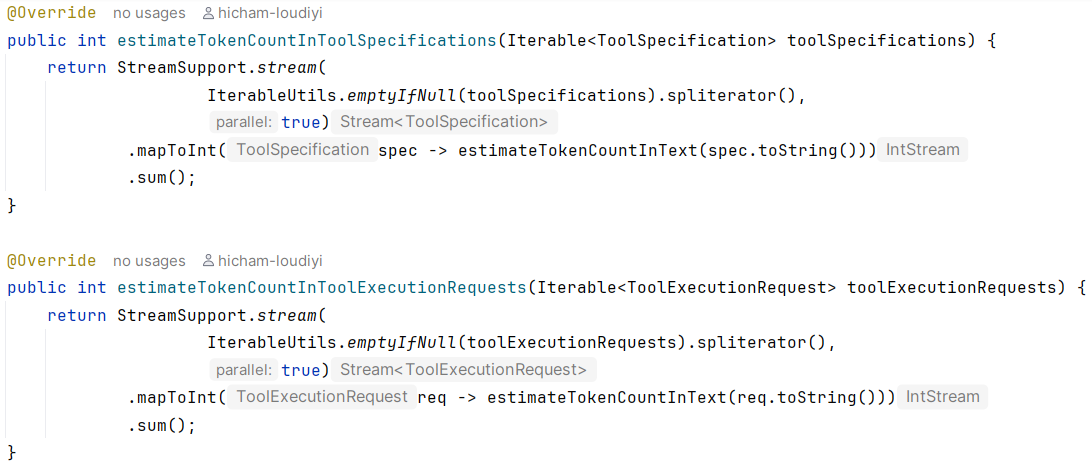
\includegraphics[width=1\textwidth]{before-factorisation.png}}
		\caption{\textit{Exemple de code répétitif avant factorisation}}
		\label{fig:before-factorisation}
	\end{figure}
	
	Dans la figure \ref{fig:before-factorisation}, chacune des méthodes \verb|estimateTokenCountInToolSpecifications| et \verb|estimateTokenCountInToolExecutionRequests| permet d'utiliser un Stream pour estimer un nombre de tokens sur un itérable, c'est donc une logique répétée, seuls le type d'objets de l'Iterable et la méthode de comptage appliquée à chaque objet sont différents. La figure \ref{fig:after-factorisation} illustre la version améliorée après factorisation.
	
	\begin{figure}[H]
		\centering
		\fbox{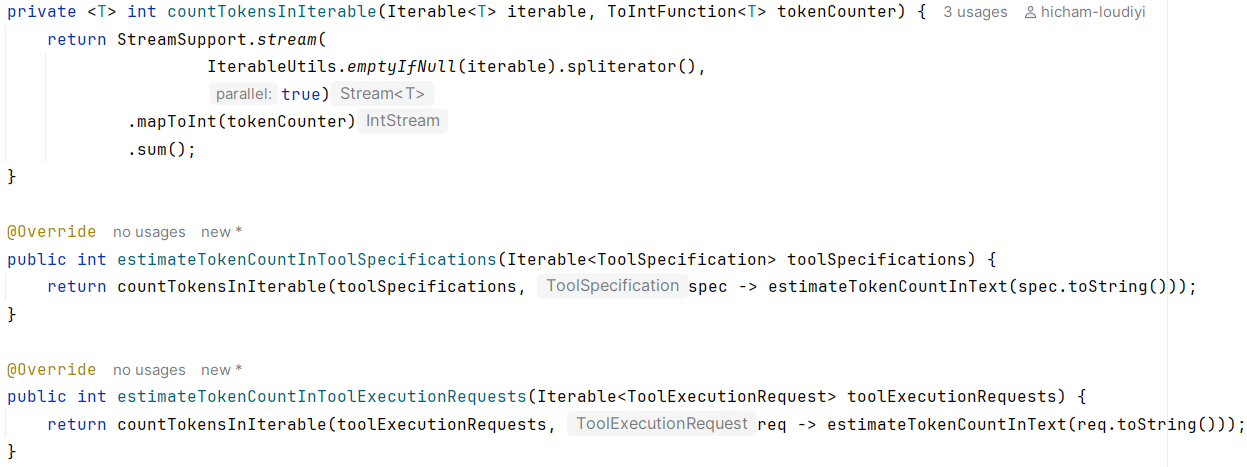
\includegraphics[width=1\textwidth]{after-factorisation.png}}
		\caption{\textit{Code refactorisé avec méthode utilitaire}}
		\label{fig:after-factorisation}
	\end{figure}
	
	La logique répétée est regroupée dans la méthode utilitaire \\ \verb|countTokensInIterable(Iterable<T> iterable, ToIntFunction<T> tokenCounter)|, puis réutilisée en appelant cette méthode au besoin.
	
	On constate une nette amélioration de la clarté du code, les règles de validation sont centralisées dans une méthode dédiée, facilitant ainsi leur réutilisation et leur évolution future.
	
	\subsection{Utilisation d'une classe de configuration}
	
	Pour standardiser et optimiser la gestion des paramètres techniques et métiers, nous avons intégré une classe de configuration nommée \verb|ConfigurationPropertyValue| dans notre projet, comme le montre la figure \ref{fig:configuration-property-value}. Dans cette classe nous avons externalisé des valeurs de configuration comme le nom du modèle de language, sa température, le maximum de messages du ChatMemory, des paramètres du Retriever, la taille maximale des images uploadées et bien d'autres. Nous avons injecté ces valeurs dans la classe - via l'annotation \verb|@Value| - dans un premier temps depuis le fichier de configuration \verb|application.properties|, et nous avons basculé ensuite vers une base de données. L'annotation \verb|@Value| offre la possibilité de définir des valeurs par défaut en cas d'absence de valeurs à injecter.
	
	\begin{figure}[H]
		\centering
		\fbox{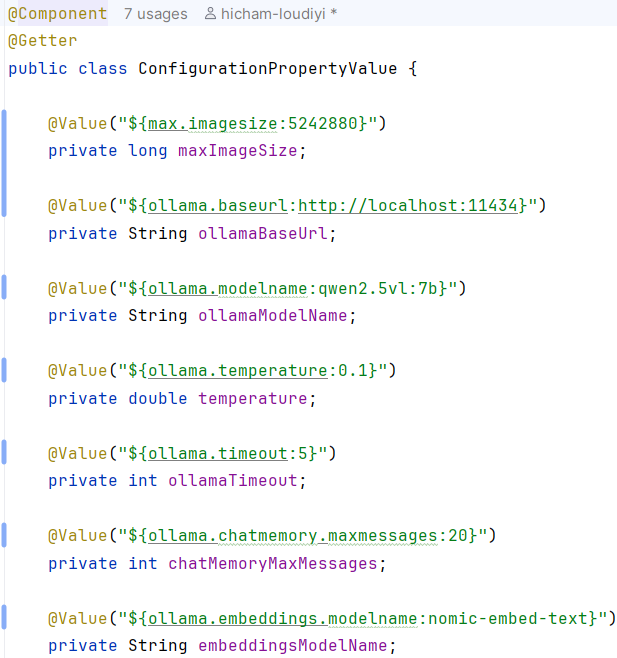
\includegraphics[width=0.7\textwidth]{configuration-property-value.png}}
		\caption{\textit{Un morceau de la classe de configuration}}
		\label{fig:configuration-property-value}
	\end{figure}
	
	Pour récupérer ces valeurs dans une autre classe, il suffit d'y injecter un bean de la classe de configuration, comme le montre l'exemple dans la figure \ref{fig:using-configuration-property-value}.
	
	\begin{figure}[H]
		\centering
		\fbox{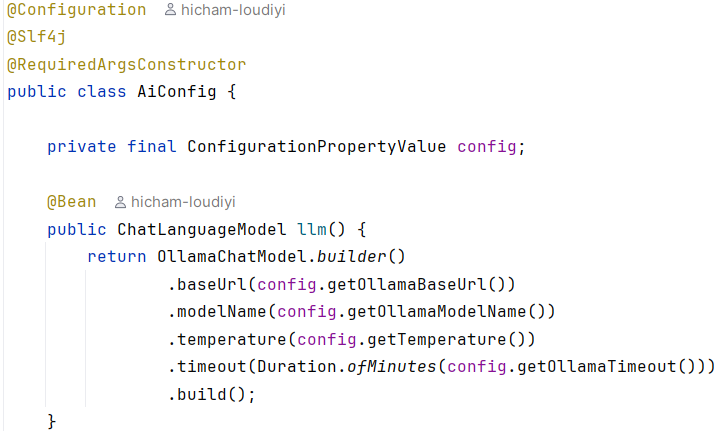
\includegraphics[width=0.8\textwidth]{using-configuration-property-value.png}}
		\caption{\textit{Utilisation de la classe de configuration}}
		\label{fig:using-configuration-property-value}
	\end{figure}
	
	Avec cette approche on peut ajuster les paramètres techniques sans toucher au code métier et sans recompilation, on gagne plus de flexibilité en adaptant les paramètres à l'environnement (dev, test, prod) via des profils Spring, et on respecte l'un des principe SOLID, qui est la séparation des responsabilités, puisque le service se concentre sur la logique métier, tandis que la configuration technique est externalisée.
	
	\section{Interfaces graphiques réalisées}
	
	Pour atteindre nos objectifs ambitieux, nous avons suivi une approche incrémentielle. Dans un premier temps, nous avons réalisé un prototype fonctionnel afin de valider les fondements techniques du projet, de comprendre le fonctionnement du framework LangChain4j, de tester l’intégration avec Ollama, et de valider le concept de récupération de contexte à partir de documents externes.
	
	Ensuite, Nous avons procédé au développement du projet final, en orientant le premier prototype vers l'analyse et la correction des erreurs et anomalies logicielles, et en le dotant d'une dimension multimodale.
	
	\subsection{Prototype exploratoire}
	
	Le premier prototype est basé sur un agent intelligent exploitant une architecture RAG unimodale, capable de répondre aux questions de l’utilisateur à partir d’un document texte ou PDF fourni.
	
	Pour tester ce prototype, nous avons fourni à l'application le chemin d'un fichier PDF, dont le contenu est une lettre de recommandation pour une étudiante appelée Nour, nous avons ensuite posé une question à propos de cette étudiante à l'agent AI, en utilisant un contrôleur web. La figure \ref{fig:test-rag} montre le résultat obtenu.
	
	\begin{figure}[H]
		\centering
		\fbox{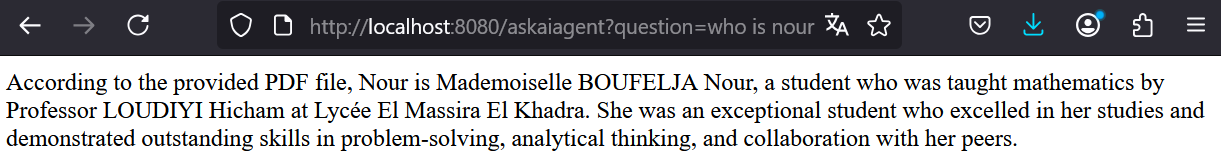
\includegraphics[width=\textwidth]{test-rag.png}}
		\caption{\textit{Test du premier prototype}}
		\label{fig:test-rag}
	\end{figure}
	
	Le modèle de language que nous avons choisi pour tester ce prototype est Llama3, le prototype à réussi à répondre correctement à la question posée.
	
	\subsection{Version livrable actuelle}
	
	\subsubsection{Structure du projet Java}
	
	Une bonne structuration d’un projet logiciel constitue un fondement essentiel pour assurer sa lisibilité, sa maintenabilité et son évolutivité. Dans notre cas, le projet respecte les conventions standard de l’écosystème Java et de l’architecture Spring Boot. L’arborescence capturée dans la figure \ref{fig:structure-projet} suit une séparation claire entre les différentes couches de l’application, notamment les agents (\verb|agents|), la configuration (\verb|config|), les objets de transfert de données (\verb|dto|), les exceptions personnalisées (\verb|exceptions|), les services métier (\verb|service|) et la couche de présentation via les contrôleurs web (\verb|web|). Par cette organisation modulaire, nous avons favorisé l'encapsulation des responsabilités, en conformité avec les principes SOLID, et facilité les tests unitaires ainsi que l’intégration continue. Par ailleurs, l’intégration des ressources statiques et de configuration dans les répertoires \verb|resources|/\verb|static| et \verb|application.properties| respecte les conventions de Spring Boot, permettant un déploiement harmonisé (voir la page 43).
	
	\begin{figure}[H]
		\centering
		\fbox{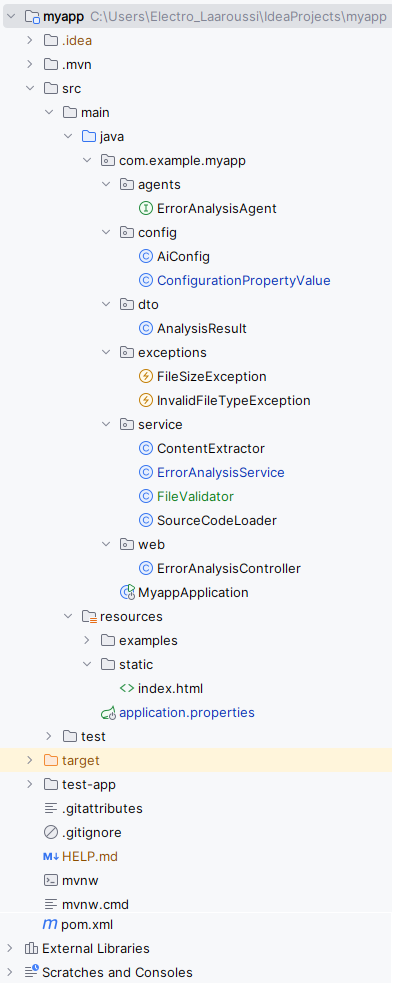
\includegraphics[width=0.57\textwidth]{structure-projet.png}}
		\caption{\textit{Structure du projet Java}}
		\label{fig:structure-projet}
	\end{figure}
	
	\subsubsection{Configuration des modèles et chargement des ressources pour le RAG}
	
	Afin de permettre à notre application de traiter des entrées de natures hétérogènes (texte, image, vidéo), le recours à un modèle de langage multimodal s’est révélé indispensable. À cet effet, nous avons choisi le modèle \verb|Qwen2.5vl:7b| pour ses capacités avancées d’analyse conjointe du contenu textuel et visuel.
	
	Nous avons aussi configuré plusieurs autres paramètres, telles que les paramètres relatifs au LLM, au modèle d'Embeddings, et au Retriever.
	
	Les images de grande taille entraînent une diminution significative des performances en raison de leur impact sur la vitesse de transfert réseau, le temps de décodage en base64, ainsi que sur l'efficacité de l'analyse par le modèle de langage. Cette contrainte nous a conduit à imposer une limite stricte à leur taille maximale.
	
	D'autre part, nous avons configuré le service \verb|sourceCodeLoader| à charger les fichiers du code source de l'application présentant des erreurs, en lui disposant de son chemin. Ces fichiers constituent la matière première pour le RAG, qui les utilisera pour enrichir sa base de connaissances, afin d'obtenir des réponses cohérentes avec le contexte de l'application à déboguer.
	
	Nous avons défini toutes les valeurs de ces configuration - en premier lieu - dans le fichier \verb|application.properties|, comme l'illustre la figure \ref{fig:properties} (voir la page 45).
	
	\begin{figure}[H]
		\centering
		\fbox{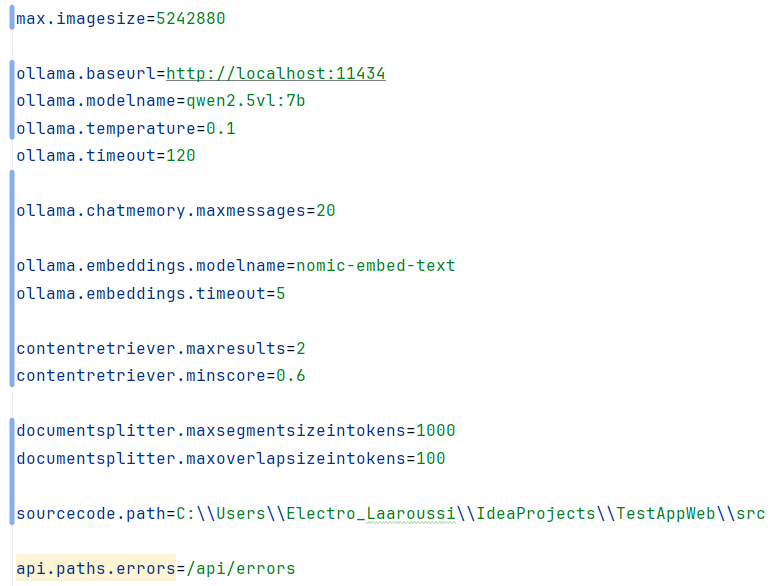
\includegraphics[width=0.8\textwidth]{properties.png}}
		\caption{\textit{Morceau du contenu du fichier application.properties}}
		\label{fig:properties}
	\end{figure}
	
	Par ailleurs, comme montré dans la figure \ref{fig:ai-agent} nous avons configuré l'agent AI pour définir son rôle, et pour lui décrire précisément l'input de l'utilisateur et qu'on attend de l'agent (voir la page 46).
	
		\begin{figure}[H]
		\centering
		\fbox{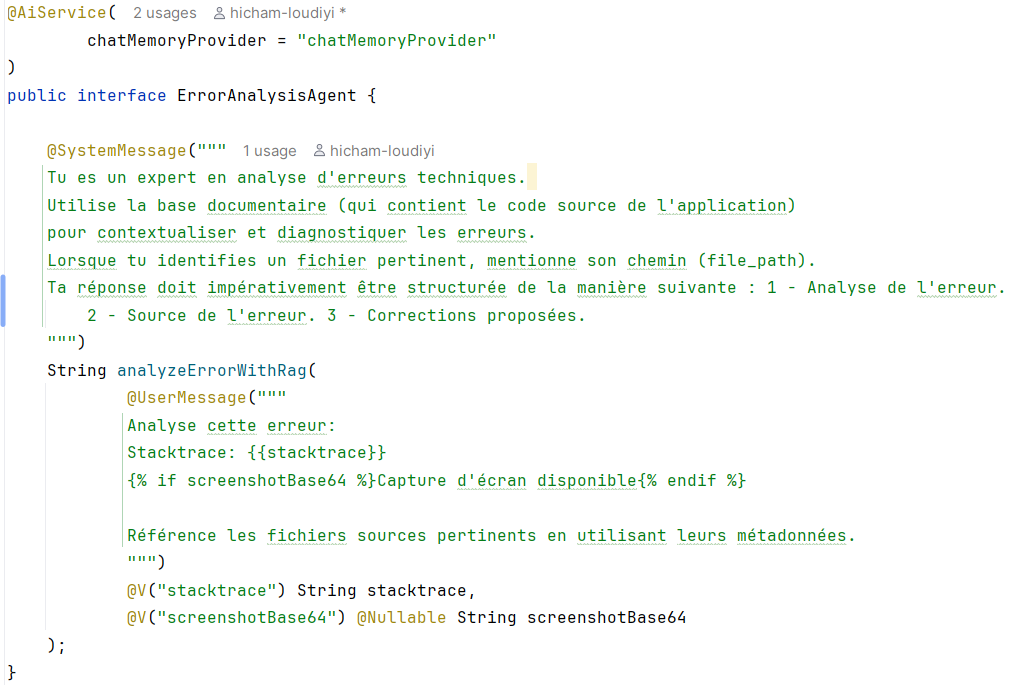
\includegraphics[width=1\textwidth]{ai-agent.png}}
		\caption{\textit{Interface Java de l'agent AI}}
		\label{fig:ai-agent}
	\end{figure}
	
	\subsubsection{Démarrage de l'Application Spring Boot}
	
	Au démarrage de l'application, Spring Boot initialise le contexte d'exécution en suivant une séquence bien définie. Tout commence par le chargement de la classe principale \verb|MyappApplication|, annotée avec \verb|@SpringBootApplication|, qui active la configuration automatique, la scan des composants et les propriétés définies dans \verb|application.properties|. Les beans déclarés dans \verb|AiConfig| sont instanciés, configurant notamment le modèle RAG et les services dépendants comme \verb|ErrorAnalysisAgent| ou \verb|SourceCodeLoader|. En parallèle, Spring MVC s'initialise pour préparer les endpoints du contrôleur \\ \verb|ErrorAnalysisController|. Enfin, le serveur embarqué Tomcat démarre et expose l'API sur le port configuré, rendant accessible l'interface Swagger UI pour tester les endpoints. Cette orchestration garantit que tous les services et composants sont prêts à traiter les requêtes dès le démarrage complet.
	
	\subsubsection{Conformité aux Normes RESTful et Bonnes Pratiques d'API}
	
	Notre projet respecte les principes fondamentaux d'une API RESTful. En effet L'endpoint \verb|/api/errors| suit une sémantique HTTP claire, la méthode POST est utilisée pour la création d'une ressource, conformément aux verbes REST, et les réponses HTTP sont standardisées (200 pour le succès, 400/413/415/500 pour les erreurs métier) avec des codes de statut pertinents et des messages structurés dans le DTO \verb|AnalysisResult|. L'utilisation de \verb|@RestController| et de \\ \verb|MediaType.MULTIPART_FORM_DATA_VALUE| garantit une sérialisation/désérialisation transparente des données. [4]
	
	De plus, l'API développée est documentée via Swagger/OpenAPI (à l'aide des annotations \verb|@Tag|, \verb|@Operation|),offrant une spécification interactive des endpoints, des schémas de requête/réponse, et des codes d'erreur. La gestion des données binaires (comme les captures d'écran via \verb|MultipartFile|) et leur validation rigoureuse (contrôle de la taille maximale et des types MIME autorisés) respectent les bonnes pratiques RESTful pour les formats de données complexes. [5]
	
	\subsubsection{Création d'une page web pour effectuer des tests}
	
	Nous avons conçu une interface web minimaliste (figure \ref{fig:interface}) permettant de soumettre les erreurs rencontrées dans les applications. Cette page offre un formulaire où l'utilisateur peut soumettre une description détaillée - et/ou une stacktrace  - du problème ainsi qu’une capture d’écran optionnelle illustrant l’anomalie, un bouton "Analyser l'erreur", et un champs de texte où la réponse générée va être affichée.
	
	\begin{figure}[H]
		\centering
		\fbox{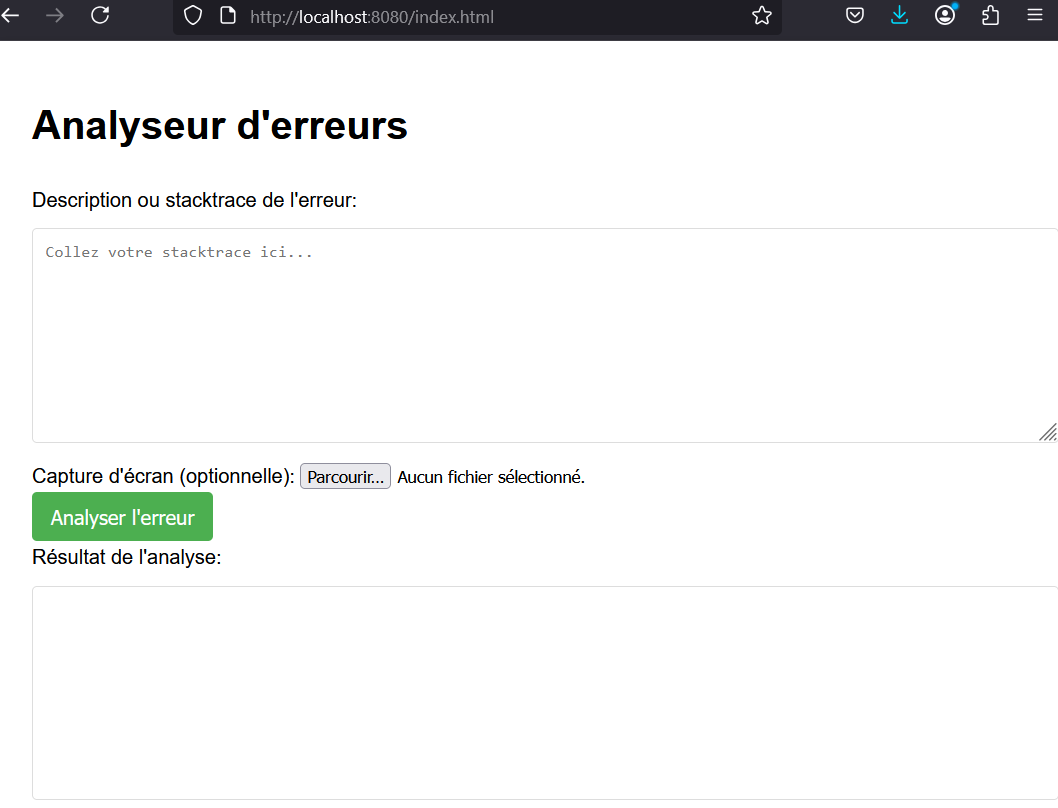
\includegraphics[width=\textwidth]{interface.png}}
		\caption{\textit{Interface de l'application de test}}
		\label{fig:interface}
	\end{figure}
	
	
	\subsubsection{Simulation d'une application qui génère une erreur}
	
	Afin de simuler un cas réel d'erreur dans une application, nous avons développé une application web de test générant intentionnellement une exception de type \verb|NullPointerException|. Ce type d'exceptions - fréquent dans le développement logiciel - se produit lorsqu'une méthode tente d'accéder à un objet non initialisé (\verb|null|). La figure \ref{fig:simulation-erreur} montre le résultat de l'exécution sur un navigateur.
	
	\begin{figure}[H]
		\centering
		\fbox{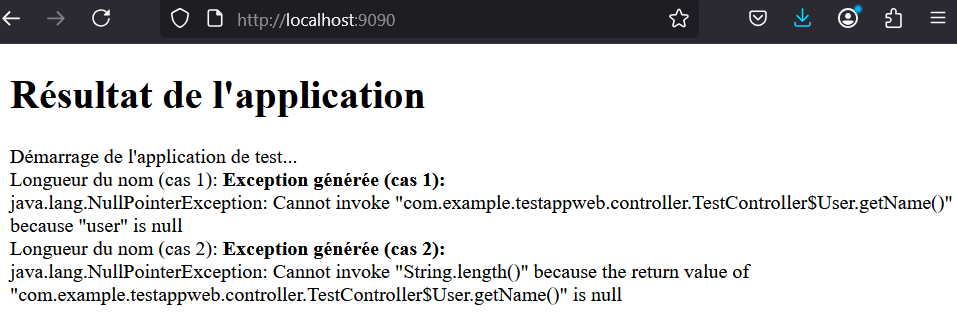
\includegraphics[width=\textwidth]{simulation-erreur.png}}
		\caption{\textit{Résultat d'exécution de l'application de test}}
		\label{fig:simulation-erreur}
	\end{figure}
	
	\subsubsection{Une analyse réussie}
	
	Nous avons soumis la capture d'écran dans la figure \ref{fig:simulation-erreur} à notre analyseur d'erreurs avec une petite description, ainsi que le chemin vers son code source (récupéré par RAG). Après une dizaine de secondes, la réponse est affichée, comme illustré dans la figure \ref{fig:premier-test} (voir la page 50).
	
	\begin{figure}[H]
		\centering
		\fbox{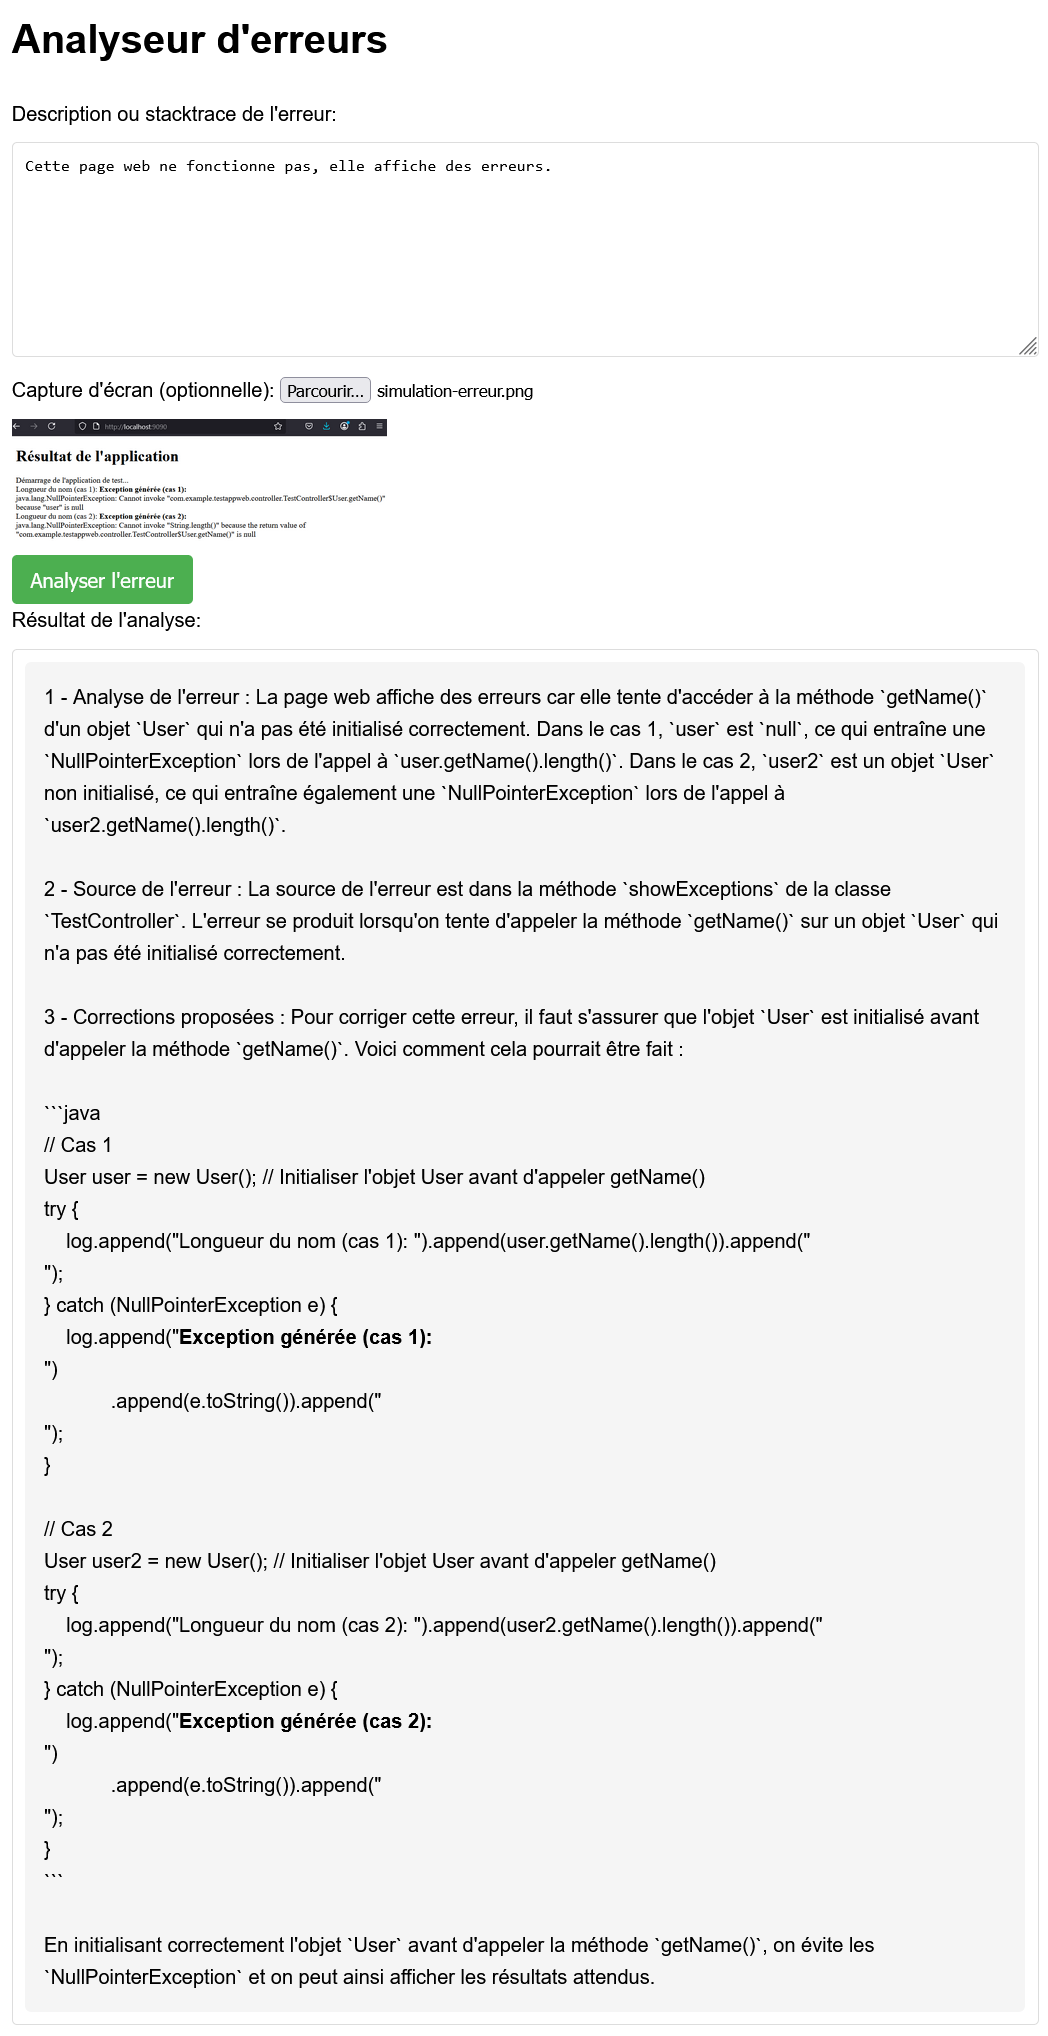
\includegraphics[width=0.75\textwidth]{premier-test.png}}
		\caption{\textit{Résultat d'une analyse d'erreur réussie}}
		\label{fig:premier-test}
	\end{figure}
	
	La réponse du système montre qu'il a correctement compris la requête, chargé la base de conaissances (code source), identifié l'erreur et sa cause, et proposé des correctifs. 
	
	Nous avons testé l'ensemble des endpoints de l'API avec succès via l'interface Swagger UI, qui a permis de simuler des requêtes HTTP dans différents scénarios d'utilisation. Les réponses retournées ont été systématiquement vérifiées en termes de structure, de code de statut, et de contenu. Par exemple, la figure \ref{fig:swagger-ui} illustre le cas d'une analyse réussie, avec un code d'état \verb|200| (voir la page 52).
	
	\begin{figure}[H]
		\centering
		\fbox{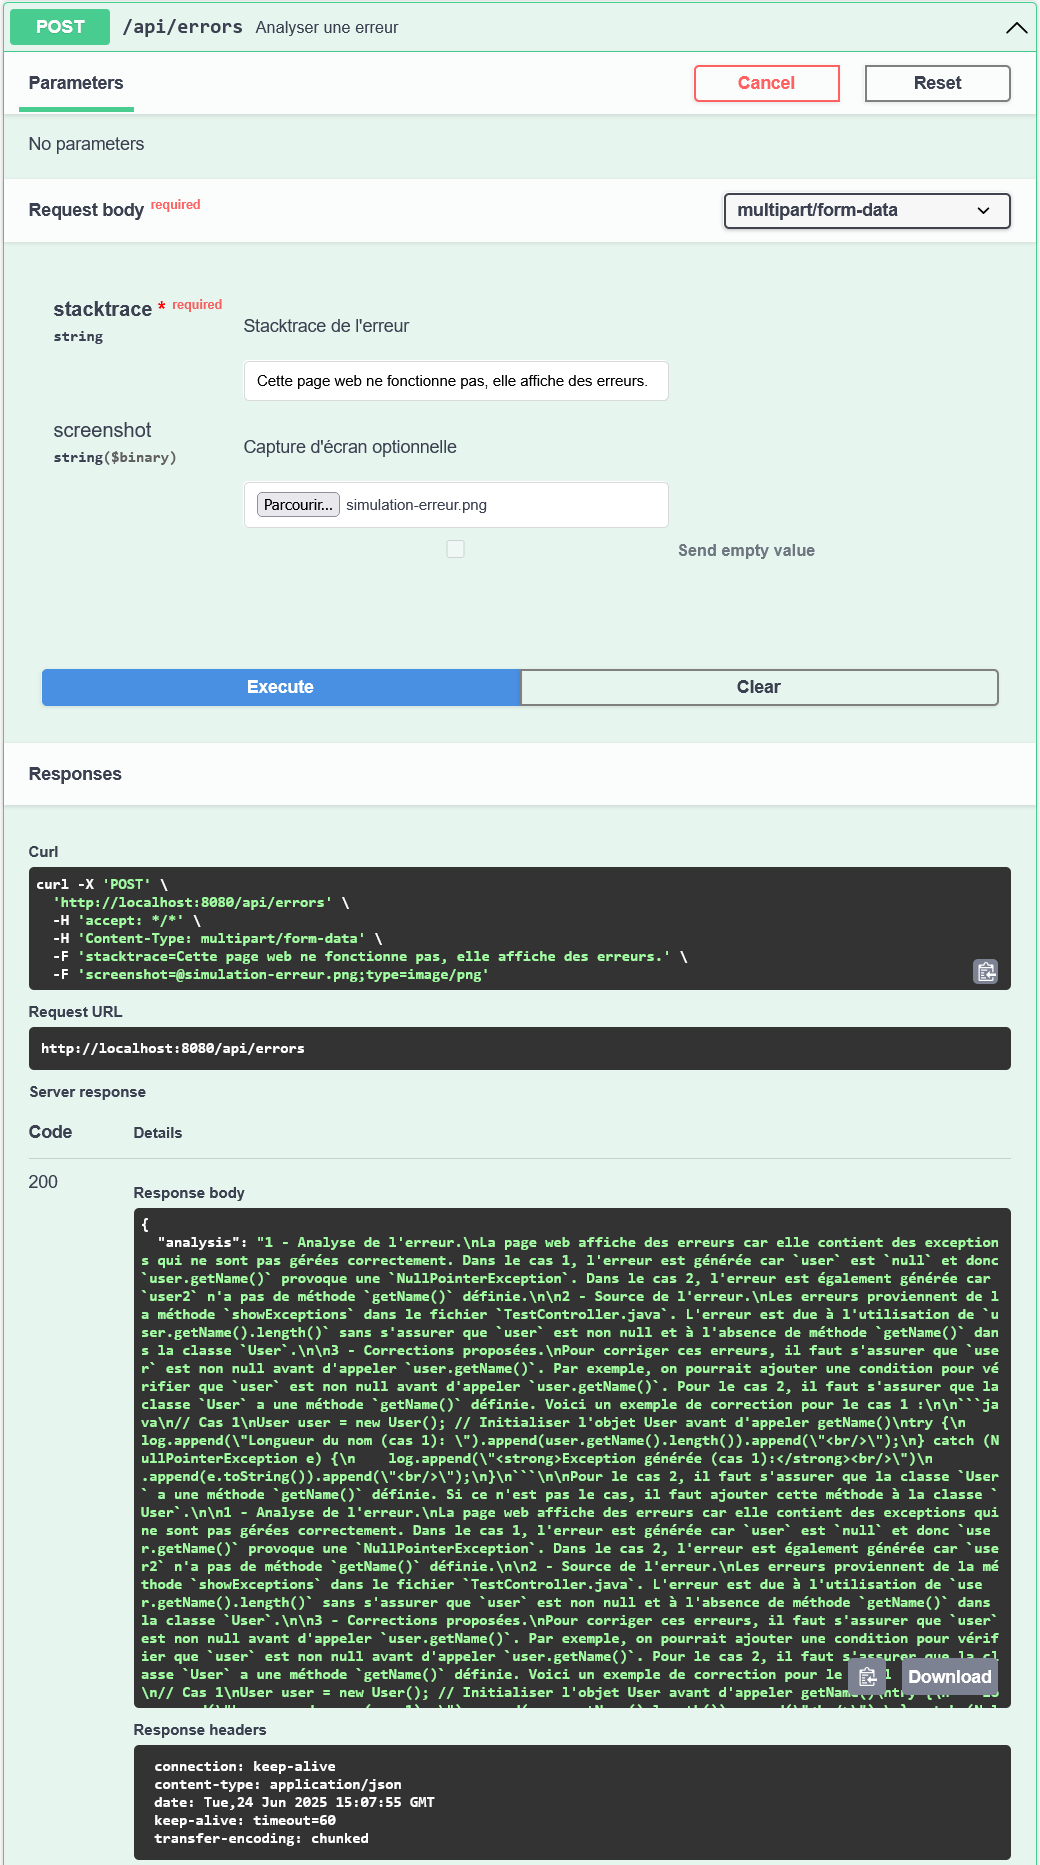
\includegraphics[width=0.8\textwidth]{swagger-ui.png}}
		\caption{\textit{Interface Swagger UI}}
		\label{fig:swagger-ui}
	\end{figure}
	
	\subsubsection{Test d'upload d'une image trop volumineuse}
	
	Pour assurer la protection du système contre la surcharge en cas d'upload d'une image de taille supérieure à celle définie dans le paramètre \verb|max.imagesize|, l'API bloque la requête en retournant le code d'état \verb|413|, comme illustré dans la figure \ref{fig:image-tros-grande}.
	
	\begin{figure}[H]
		\centering
		\fbox{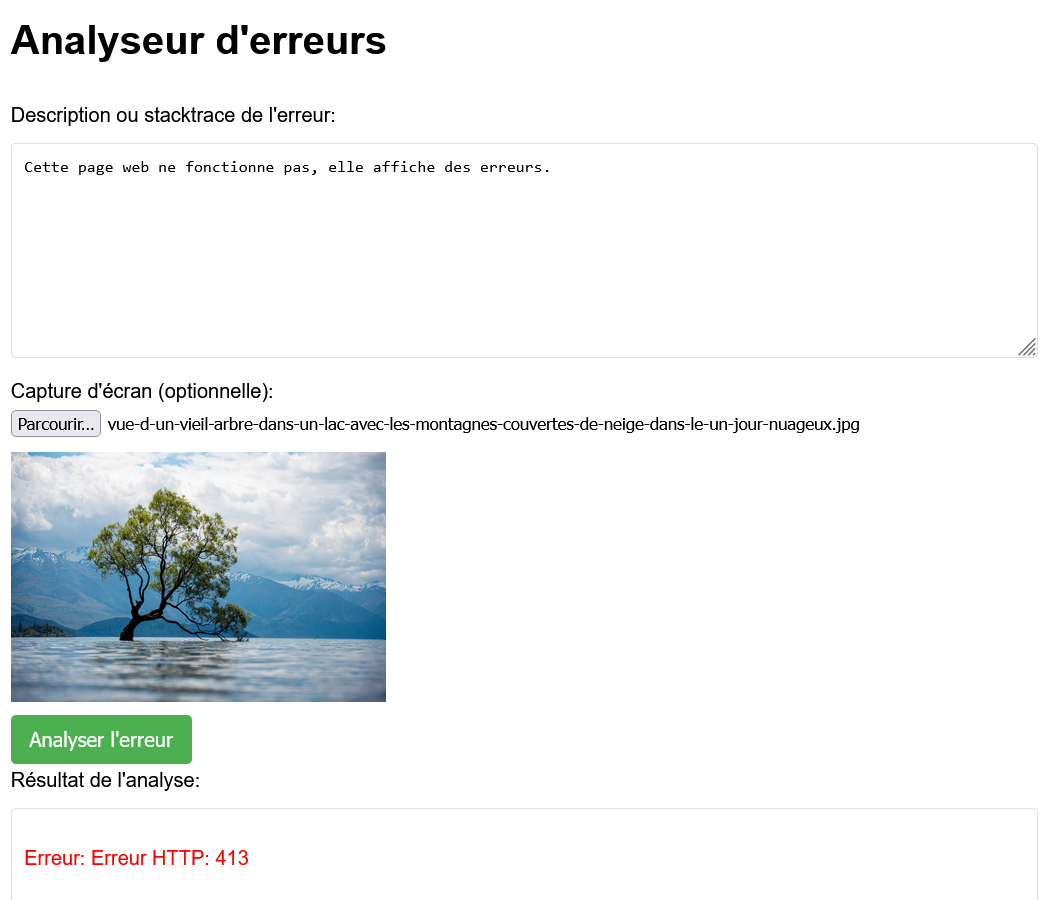
\includegraphics[width=0.8\textwidth]{image-tros-grande.png}}
		\caption{\textit{Image trop volumineuse}}
		\label{fig:image-tros-grande}
	\end{figure}
	
	\subsubsection{Test d'upload d'une image de format non supporté}
	
	Pour éviter de surcharger inutilement notre système, l'API bloque les requêtes contenant des fichiers non supportés, et retourne le code d'état \verb|415|, comme le montre la figure \ref{fig:format-non-supporté}.
	
	\begin{figure}[H]
		\centering
		\fbox{\includegraphics[width=0.8\textwidth]{format-non-supporté.png}}
		\caption{\textit{Type d'image non supporté}}
		\label{fig:format-non-supporté}
	\end{figure}
	
	\subsubsection{Prise en charge des vidéos}
	
	Dans certains cas, une erreur ou une anomalie survenue au sein d’un système est plus efficacement illustrée par une capture vidéo. A cet effet nous avons enrichi notre système par l’ajout d’une fonctionnalité permettant le téléversement de vidéos, en intégrant un nouveau service nommé \verb|VideoProcessor|. Nous avons conçu ce service de manière à ce qu'il soit capable d'extraire automatiquement des images clés à partir des vidéos fournies, via une bibliothèque appelée \verb|FFmpeg|, facilitant ainsi l’analyse des dysfonctionnements observés.
	
	La figure \ref{fig:video} illustre le résultat de l'upload d'une vidéo capturée au moment d'essayer d'atteindre une page web qui finit par afficher des stacktraces d'erreurs.
	
	\begin{figure}[H]
		\centering
		\fbox{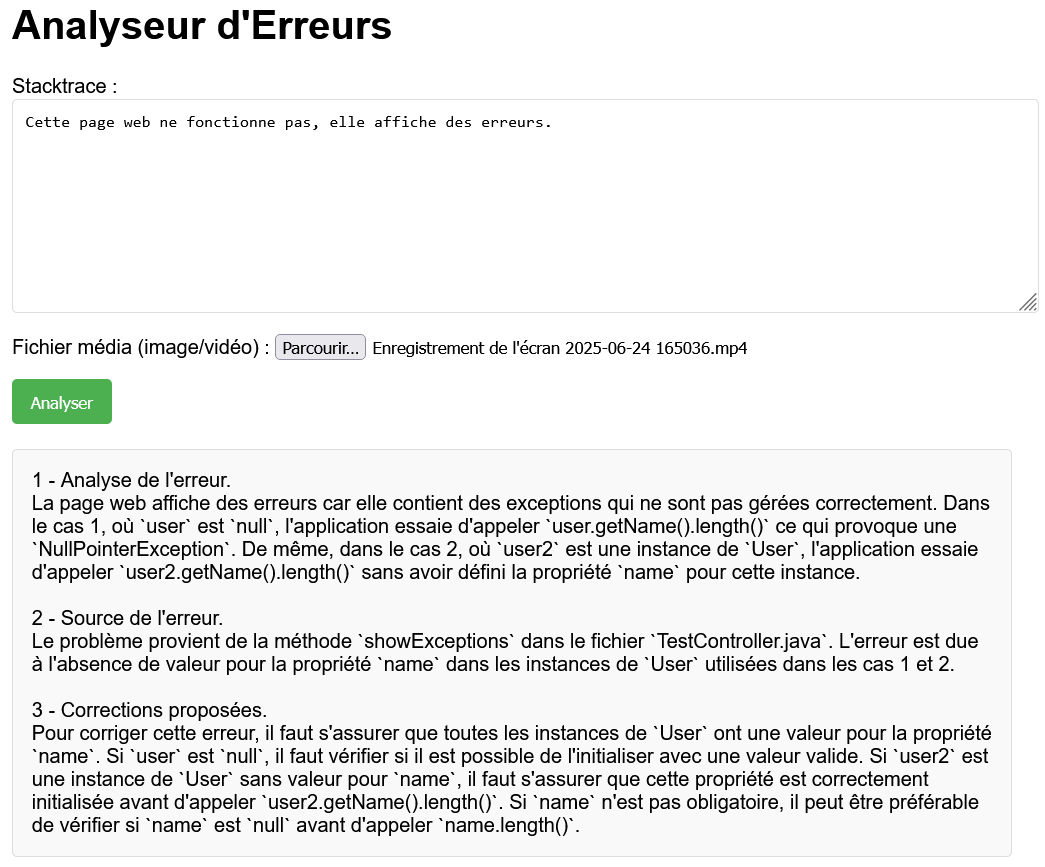
\includegraphics[width=0.8\textwidth]{video.png}}
		\caption{\textit{Upload de vidéo}}
		\label{fig:video}
	\end{figure}
	
	La réponse obtenue lors de ce test, montre que notre système a bien identifié l'erreur et sa source, mais la correction qu'il a proposée est moins pertinente puisqu'il n'a pas suggéré des morceaux de code alternatifs.
	
	\section{Conclusion}
	
	La phase de réalisation nous a permis de concrétiser les spécifications techniques et fonctionnelles définies précédemment, en transformant les modèles conceptuels en un produit opérationnel. Grâce à une méthodologie de développement agile, chaque itération a contribué à l’enrichissement progressif du système. L’adoption de bonnes pratiques de codage, couplée à des outils de gestion de version et d’intégration continue, a assuré une base code robuste et maintenable. Les défis techniques rencontrés ont été résolus par des solutions optimisées, renforçant ainsi la fiabilité de l’application. Cette étape a non seulement validé les choix architecturaux initiaux, mais a également démontré la capacité du système à répondre aux exigences métiers, ouvrant la voie aux phases de déploiement et d’exploitation.
	
	\chapter{Acquis du Projet de Fin d'Études}
	
	Ce stage de fin d'études m'a offert une opportunité enrichissante de développer un large éventail de compétences, aussi bien sur le plan technique que dans les domaines de la gestion de projet et des interactions professionnelles.
	
	\section{Volet technique}
	
	Sur le plan technique, ce stage m’a permis d’explorer des domaines et des outils que je n’avais jamais abordés auparavant.
	
	Tout d’abord, la compétence principale acquise au cours de cette expérience est la maîtrise du RAG, une technique avancée d’IA générative. La mise en œuvre concrète de cette approche dans un projet réel m’a permis d’en comprendre pleinement les mécanismes, notamment grâce à l’utilisation de la bibliothèque \texttt{LangChain4j}.
	
	Ensuite, j’ai approfondi mes connaissances dans le développement d’applications backend en Java, notamment à travers le framework \texttt{Spring Boot}, que j’ai utilisé pour concevoir des services robustes, configurables et modulaires. Cette expérience m’a ainsi permis de mieux appréhender les architectures modernes et l’intégration de composants d’intelligence artificielle dans un contexte professionnel.
	
	\section{Volet gestion de projet}
	
	Du point de vue de gestion de projet, ce stage m’a permis de travailler dans un cadre organisationnel structuré, fondé sur le framework \texttt{Scrum}, largement adopté par l’entreprise d’accueil, Algolus.
	
	Au sein des différentes itérations (sprints), nous avons appliqué l’ensemble des pratiques agiles : réunions quotidiennes, envois de rapports journaliers, \textit{backlog refinement}, \textit{technical refinement}, \textit{sprint review}, \textit{rétrospective} et \textit{planification de sprint}. Cette rigueur dans l’application de Scrum a contribué à améliorer significativement la productivité de l’équipe et la qualité des livrables.
	
	Par ailleurs, Algolus utilise également le Lean Management, dont les méthodes comme la Résolution de Problème (RdP) ont contribué à accroître notre productivité.
	
	\chapter*{Conclusion générale et perspectives}
	\addcontentsline{toc}{chapter}{Conclusion générale et perspectives}
	
	\section*{Conclusion générale}
	\addcontentsline{toc}{section}{Conclusion générale}
	
	Ce projet a consisté en la conception et le développement d'une application dédiée à l'analyse automatique d'erreurs et anomalies, intégrant une approche innovante combinant traitement multimédia (images et vidéos) et intelligence artificielle à dimension multimodale. À travers une architecture modulaire basée sur Spring Boot et une interface web interactive, le système offre une solution robuste pour diagnostiquer des anomalies logicielles et proposer des corrections contextualisées.
	
	Les principaux objectifs fixés ont été atteints :  
	
	\begin{itemize}
		
		\item \textbf{Fonctionnalité de base} : L'application analyse efficacement les stacktraces,  identifie les sources d'erreurs et suggère des correctifs grâce à une intégration réussie avec un modèle LLM (Ollama).
		
		\item \textbf{Support multimodal} : L'extension pour traiter des captures d'écran et des extraits vidéo ajoute une dimension visuelle à l'analyse, améliorant la précision des diagnostics.
		
		\item \textbf{Expérience utilisateur} : L'interface intuitive permet aux développeurs de soumettre facilement leurs erreurs et de recevoir des réponses structurées.
		
	\end{itemize}

	L'implémentation a mis en œuvre des bonnes pratiques logicielles :
	
	\begin{itemize}
		
		\item \textbf{Backend} : Architecture RESTful avec Spring Boot, validation des entrées, gestion des erreurs granulaires, et documentation OpenAPI.
		
		\item \textbf{Frontend} : Interface responsive avec gestion dynamique des médias et feedback visuel.
		
		\item \textbf{Intégration IA} : Utilisation de RAG pour contextualiser les analyses avec la base de code source. 
		
	\end{itemize}
	
	\section*{Perspectives}
	\addcontentsline{toc}{section}{Perspectives}
	
	Comme tout projet informatique, notre solution présente à la fois certaines limitations inhérentes à sa conception actuelle et des perspectives d'amélioration qui ouvrent la voie à des évolutions futures.
	
	Les pistes d'amélioration incluent :
	
	\begin{itemize}
		
		\item L'ajout d'un deuxième agent AI qui a pour rôle de juger la pertinence des réponses et/ou leur respect de certaines normes (RGPD par exemple).
		
		\item L’intégration d’un fine-tuning du modèle sur des bases de code spécifiques.
		
		\item L'ajout d'un système d'authentification pour un suivi personnalisé des analyses.
		
		\item  L'intégration avec des plateformes comme GitHub pour une analyse directe des dépôts. 
		
		\item L'amélioration des prompts IA pour couvrir un spectre plus large d'erreurs.
	
		\item L'optimisation des performances via le caching des analyses récurrentes.
		
	\end{itemize}
	
	\clearpage
	
	\begin{thebibliography}{9}
		\addcontentsline{toc}{chapter}{Bibliographie}
		
		\bibitem{rag}
		Lewis, P. et al., \emph{Retrieval-Augmented Generation for Knowledge-Intensive NLP Tasks}, arXiv, 2020.\\
		\url{https://arxiv.org/abs/2005.11401}
		
	\end{thebibliography}
	
	% Webographie (sites, documentations en ligne)
	\chapter*{Webographie}
	\addcontentsline{toc}{chapter}{Webographie}
	
	\begin{enumerate}[label=\textbf{[\arabic*]}, start=2]
		\item Ollama, \emph{Model Library}, 2023. \\
		\url{https://ollama.ai/library}
		
		\item Oracle, \emph{Package java.util.stream}, 2021. \\
		\url{https://docs.oracle.com/en/java/javase/17/docs/api/java.base/java/util/stream/package-summary.html}
		
		\item Spring Team, \emph{Building REST Services with Spring}, 2023. \\
		\url{https://spring.io/guides/gs/rest-service/}
		
		\item OpenAPI Initiative, \emph{OpenAPI Specification}, 2023. \\
		\url{https://swagger.io/specification/}
	\end{enumerate}
	
	\chapter*{Annexes}
	\addcontentsline{toc}{chapter}{Annexes}
	
	\section*{Evaluation des objectifs}
	\addcontentsline{toc}{section}{Evaluation des objectifs}
	
	\subsection*{Méthodologie d'évaluation}
	
	
	Pour mesurer l’efficacité du système, nous avons mené des tests sur un échantillon d'erreurs courantes (de types \verb|NullPointerException|, \verb|ArrayIndexOutOfBoundsException|, Memory Leaks, etc.), en comparant les résultats de l’outil avec ceux d’une analyse humaine. Les critères d’évaluation incluaient la précision de détection, la pertinence des correctifs, et le gain de temps.
	
	\subsection*{Résultats obtenus}
	
	
	Après effectué les tests d'évaluation des objectifs sur un échantillon de 30 erreurs, les métriques obtenues sont :
	
	\begin{itemize}
		
		\item \textbf{Taux de détection : 78\%} (proche de l’objectif de 80\%).
		
		Cela s'explique par le fait que les erreurs complexes ou dépendantes du contexte métier ont réduit la précision. Notre système montre cependant des performances supérieures sur les erreurs syntaxiques et les crashes simples.
		
		\item \textbf{Correctifs pertinents : 65\%} (objectif de 70\% partiellement atteint).
		
		Les corrections nécessitant une refactorisation majeure ou une compréhension approfondie de l’architecture ne sont pas toujours proposées. L’outil excelle sur les correctifs localisés.
		
		\item \textbf{Gain de temps : 35\%} (objectif dépassé).
		
		L’automatisation réduit significativement le temps de diagnostic, surtout pour les erreurs récurrentes. Cependant, les cas complexes nécessitent toujours une intervention humaine.
		
	\end{itemize}
	
	\section*{Benchmark de LLMs Multimodaux}
	\addcontentsline{toc}{section}{Benchmark de LLMs Multimodaux}
	
	Nous avons mené une comparaison entre trois modèles de languages multimodaux disponibles via Ollama, qui sont \verb|llava|, \verb|qwen2.5vl:7b|, et \verb|bakllava|, selon deux critères importants : les performances (Temps de réponse, utilisation CPU/RAM), et la pertinence des réponses (Exactitude des diagnostics d'erreurs).
	
	La configuration matérielle utilisée est \verb|Intel(R) Core(TM) i7-10610U CPU @ 1.80GHz| \\ \verb|2.30 GHz| avec une mémoire RAM de \verb|32,0 Go|, dont \verb|16,0 Go| est partagée avec le processeur graphique \verb|Intel(R) UHD Graphics|.
	
	Nous avons préparé un jeu de données de 20 erreurs (10 Python, 10 Java) avec stacktraces + 5 captures d’écran.
	
	\subsection*{Résultats synthétiques}
	
	Nous avons synthétisé les métriques de cette comparaison en calculant la valeur moyenne pour chaque paire LLM/critère sur le jeu de données. Le tableau \ref{tab:tableau-benchmark} présente les résultats calculés.
	
	\begin{table}[H]  
		\centering  
		\caption{\textit{Comparaison des LLMs multimodaux}}
		\label{tab:tableau-benchmark}
		\begin{tabular}{|l|c|c|c|c|}  
			\hline  
			\textbf{Modèle} & \textbf{Latence (s)} & \textbf{RAM (GB)} & \textbf{Précision (\%)} & \textbf{Pertinence} \\  
			\hline  
			LLaVA 7B & 5.4 & 6.8 & 62 & 3.2 \\  
			Qwen2.5VL:7B & 4.7 & 7.5 & 75 & 4.0 \\  
			BakLLaVA 7B & 6.2 & 8.1 & 68 & 3.8 \\  
			\hline  
		\end{tabular}  
	\end{table}
	
	\textbf{Légende} :
	
	\begin{itemize}
		
		\item Précision : \% de correctifs validés par un développeur.
		
		\item Pertinence : Note moyenne (5 = parfait).
	\end{itemize}
	
	\subsection*{Analyse des résultats}
	
	\subsubsection*{Performances}
	\begin{itemize}
		\item \verb|qwen2.5vl| est le plus rapide (4.7s) grâce à son optimisation pour les CPUs modestes.
		\item \verb|BakLLaVA| consomme plus de RAM (8.1 Go), limitant son usage sur machines légères.
	\end{itemize}
	
	\subsubsection*{Qualité des Réponses}
	\begin{itemize}
		\item \verb|qwen2.5vl| excelle en précision (75\%), notamment pour les erreurs Python.
		\item \verb|LLaVA| fournit des réponses moins précises mais acceptables en temps réel.
	\end{itemize}
	
	\subsection*{Visualisation des Performances}
	
	\begin{figure}[h]
		\centering
		\begin{tikzpicture}
			\begin{axis}[
				title={Latence des modèles},
				ybar,
				ymin=0,
				ylabel={Temps (secondes)},
				xlabel={Modèles},
				symbolic x coords={LLaVA, Qwen2.5VL, BakLLaVA},
				xtick=data,
				nodes near coords,
				bar width=0.5cm
				]
				\addplot coordinates {(LLaVA,5.4) (Qwen2.5VL,4.7) (BakLLaVA,6.2)};
			\end{axis}
		\end{tikzpicture}
		\caption{\textit{Comparaison des temps de réponse moyens}}
		\label{fig:latence}
	\end{figure}
	
	\begin{figure}[H]
		\centering
		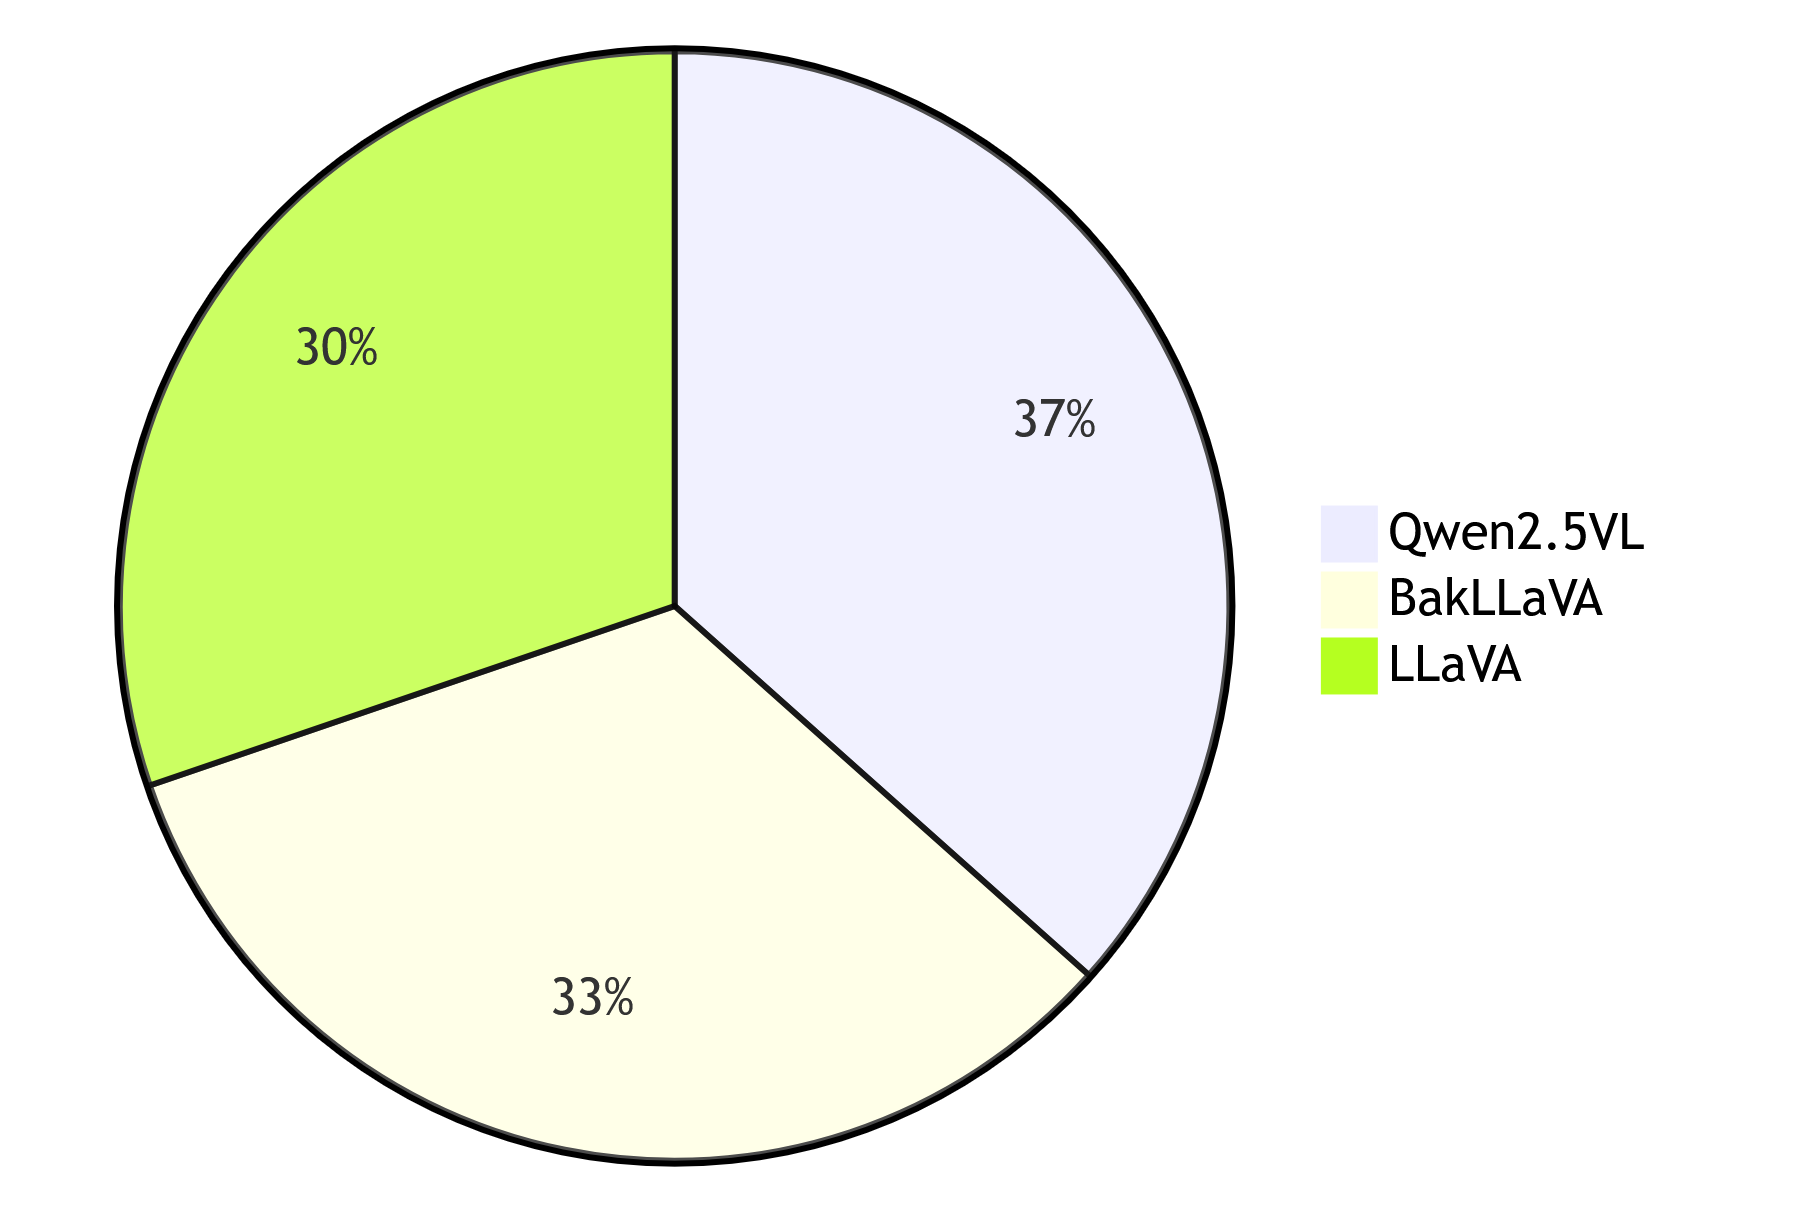
\includegraphics[width=0.8\textwidth]{precision-modeles.png}
		\caption{\textit{Précision des modèles testés}}
		\label{fig:precision-modeles}
	\end{figure}
	
	\subsection*{Discussion des résultats}
	
	L'analyse comparative révèle que \verb|qwen2.5vl| constitue le meilleur compromis pour les configurations matérielles limitées, combinant une latence réduite (4.7 s) et une précision satisfaisante (75 \%), notamment pour les erreurs Python. À l'inverse, \verb|BakLLaVA|, bien que proposant des résultats plus détaillés, s'avère trop gourmand en ressources (8.1 Go de RAM), le rendant peu adapté aux machines modestes. Ces conclusions doivent néanmoins être nuancées par la taille limitée du jeu de données (20 échantillons) – une validation sur un corpus plus large serait nécessaire pour consolider ces observations. En pratique, nous recommandons d'utiliser \verb|qwen2.5vl| comme modèle par défaut pour les analyses courantes, tandis que \verb|LLaVA|, moins précis mais plus rapide, pourrait être réservé aux tests ponctuels nécessitant un temps de réponse minimal.
	
\end{document}